% Fakesection 序言之前

\RequirePackage[l2tabu, orthodox]{nag}
\RequirePackage{ifxetex}
\RequireXeTeX

\documentclass{ctexrep}

%颜色
\usepackage{xcolor}

%长度
\usepackage{printlen}
\uselengthunit{mm}

%图形
\usepackage{media9}
\usepackage{pdfpages}
\usepackage{overpic}
\usepackage{graphicx}
\graphicspath{{./src/}}
\usepackage{wallpaper}
\usepackage{wrapfig}
\usepackage{pstricks}
\usepackage{smartdiagram}
\usepackage[edges]{forest}
\usepackage{pgfplots}
\usepackage{tikz}
\usetikzlibrary{shapes.geometric}
\usetikzlibrary{calc}
\usetikzlibrary{patterns}
\usetikzlibrary{arrows}
\usetikzlibrary{shapes}
\usetikzlibrary{chains}
\usetikzlibrary{mindmap}
\usetikzlibrary{graphs}
\usetikzlibrary{decorations.text}
\usetikzlibrary{arrows.meta}
\usetikzlibrary{shadows.blur}
\usetikzlibrary{shadings}
\usepackage{scsnowman}
\usepackage{tikzpeople}
\usepackage{tikzducks}
\usepackage{flowchart}
\usepackage{ean13isbn}
\usepackage{qrcode}
\usepackage{pgf-pie}
\usepackage{pgfmath}

%表格
\usepackage{tabu}
\usepackage{longtable}
\usepackage{booktabs}
\usepackage{diagbox}
\usepackage{multicol}
\usepackage{multirow}
\usepackage{makecell}
\usepackage{fancybox}
\usepackage{colortbl}
\usepackage[minted]{tcolorbox}
\tcbuselibrary{skins}
\tcbuselibrary{breakable}
\tcbuselibrary{theorems}
\tcbuselibrary{listings}
\tcbuselibrary{xparse}
\usepackage{fvextra}
\usepackage{csvsimple}
\usepackage{siunitx}

%公式
\usepackage{amsmath}
\usepackage{amsthm}
\usepackage{amsfonts}
\usepackage{amssymb}
\usepackage{amsbsy}
\usepackage{amsopn}
\usepackage{amstext}
\usepackage{mathrsfs}
\usepackage{bm}
\usepackage{textcomp}
\usepackage{latexsym}
\usepackage{exscale}
\usepackage{relsize}
%\usepackage{xymtex}

%正文
\usepackage{fancyhdr}
\usepackage{geometry}
\usepackage{lastpage}
\usepackage{indentfirst}
\usepackage{setspace}
\renewcommand\arraystretch{1.5}
\renewcommand{\thefootnote}{\fnsymbol{footnote}}

%非正文
\usepackage{makeidx}
\makeindex
\usepackage{epigraph}
\usepackage{varwidth}

%%链接
\usepackage
[	colorlinks = true,
linkcolor = gray,
citecolor = gray,
backref=page
]{hyperref}
\usepackage{caption}
\usepackage{subcaption}
\DeclareCaptionLabelFormat{andtable}%
{#1#2~\&~\tablename\thetable}

%其它
\usepackage{atbegshi}
\usepackage{lipsum}

\csname
endofdump
\endcsname

\usepackage{microtype}

%%代码
\usepackage{minted}

%枚举%与beamer冲突
\usepackage{enumitem}
\setlist[enumerate, 2]{
	fullwidth,
	label = \alph*.,
	font = \textup,
	itemindent=2em
}

\usepackage{titlesec}
\titleformat{\chapter}{\centering\Huge\bfseries}{实验\chinese{chapter}}{4mm}{}
\titleformat{\section}{\large\bfseries}{\chinese{section}、}{1mm}{}
\titleformat{\subsection}{}{\arabic{subsection}.}{1mm}{}

\begin{document}

% Fakesection 扉页

\begin{titlepage}
	\centering
	\begin{figure}[htbp]
		\centering
		\includegraphics[width=.8\linewidth]{NJUST.ai}
		\label{fig:NJUST}
	\end{figure}

	\vspace{20mm}
	\textbf{\zihao{1}\heiti{数字逻辑电路}}

	\vspace{5mm}
	\textbf{\zihao{1}\heiti{实验报告}}

	\vspace{20mm}
	\begin{table}[htbp]
		\centering
		\zihao{3}
		\begin{longtabu}to.8\linewidth{@{}X[4,r]@{}X[c]@{}X[12,l]@{}}
			\makebox[4\ccwd][s]{学院}&:&\underline{\makebox[12\ccwd][c]{\kaishu{电子工程与光电技术学院}}}\\
			\makebox[4\ccwd][s]{班号}&:&\underline{\makebox[12\ccwd][c]{\kaishu{9171040G11}}}\\
			\makebox[4\ccwd][s]{姓名}&:&\underline{\makebox[12\ccwd][c]{\kaishu{吴振宇}}}\\
			\makebox[4\ccwd][s]{学号}&:&\underline{\makebox[12\ccwd][c]{\kaishu{916101630117}}}\\
			\makebox[4\ccwd][s]{实验编号}&:&\underline{\makebox[12\ccwd][c]{\kaishu{0450}}}\\
			\makebox[4\ccwd][s]{指导老师}&:&\underline{\makebox[12\ccwd][c]{\kaishu{谭雪琴}}}\\
		\end{longtabu}
	\end{table}

	\vspace{10mm}
	\zihao{3}
	\kaishu{\today}
\end{titlepage}

%页眉页脚%与book冲突
\pagestyle{fancy}
\renewcommand{\headrulewidth}{0pt}
\lhead{}
\chead{}
\rhead{}
\lfoot{\small{实验\chinese{chapter}}}
\cfoot{\small{第\thepage 页~共~\pageref{LastPage}~页}}
\rfoot{}

% Fakesection 目录

\pagenumbering{roman}

\tableofcontents

\newpage

\listoffigures

\newpage

\listoftables

\newpage

\pagenumbering{arabic}

\chapter{组合逻辑电路设计}%
\label{cha:组合逻辑电路设计}

\setcounter{page}{1}
\section{实验目的}%
\label{sec:实验目的\arabic{chapter}}

\begin{enumerate}
	\item 熟悉基本门电路的逻辑功能及应用;
	\item 掌握用逻辑代数或卡诺图化简逻辑表达式的方法:
	\item 理解组合逻辑电路的设计与搭建原则。
\end{enumerate}

\section{实验内容}%
\label{sec:实验内容\arabic{chapter}}

在远程实验平台\href{http://192.10.84.32/}{(e'lab)}完成以下组合逻辑电路的设计与验证:

\begin{enumerate}
	\item 用与非门和异或门设计全加器电路:
	\item 用与非门设计组合逻辑电路,其功能示意如图\ref{fig:要求}:
		\begin{figure}[htbp]
			\centering
			\begin{subfigure}[htbp]{.45\linewidth}
				\centering
				% Graphic for TeX using PGF
% Title: D:\User\Documents\Individual\Coursewares\电学\数电模电\数电 谭 课件+ewb\0450\src\12.dia
% Creator: Dia v0.97.2
% CreationDate: Tue Apr 02 23:11:46 2019
% For: Wu Zhenyu
% \usepackage{tikz}
% The following commands are not supported in PSTricks at present
% We define them conditionally, so when they are implemented,
% this pgf file will use them.
\ifx\du\undefined
  \newlength{\du}
\fi
\setlength{\du}{15\unitlength}
\begin{tikzpicture}
\pgftransformxscale{1.000000}
\pgftransformyscale{-1.000000}
\definecolor{dialinecolor}{rgb}{0.000000, 0.000000, 0.000000}
\pgfsetstrokecolor{dialinecolor}
\definecolor{dialinecolor}{rgb}{1.000000, 1.000000, 1.000000}
\pgfsetfillcolor{dialinecolor}
\definecolor{dialinecolor}{rgb}{1.000000, 1.000000, 1.000000}
\pgfsetfillcolor{dialinecolor}
\fill (17.807500\du,14.600000\du)--(17.807500\du,17.300000\du)--(21.692500\du,17.300000\du)--(21.692500\du,14.600000\du)--cycle;
\pgfsetlinewidth{0.100000\du}
\pgfsetdash{}{0pt}
\pgfsetdash{}{0pt}
\pgfsetmiterjoin
\definecolor{dialinecolor}{rgb}{0.000000, 0.000000, 0.000000}
\pgfsetstrokecolor{dialinecolor}
\draw (17.807500\du,14.600000\du)--(17.807500\du,17.300000\du)--(21.692500\du,17.300000\du)--(21.692500\du,14.600000\du)--cycle;
% setfont left to latex
\definecolor{dialinecolor}{rgb}{0.000000, 0.000000, 0.000000}
\pgfsetstrokecolor{dialinecolor}
\node at (19.750000\du,15.700000\du){组合逻辑};
% setfont left to latex
\definecolor{dialinecolor}{rgb}{0.000000, 0.000000, 0.000000}
\pgfsetstrokecolor{dialinecolor}
\node at (19.750000\du,16.500000\du){电路};
\pgfsetlinewidth{0.100000\du}
\pgfsetdash{}{0pt}
\pgfsetdash{}{0pt}
\pgfsetbuttcap
{
\definecolor{dialinecolor}{rgb}{0.000000, 0.000000, 0.000000}
\pgfsetfillcolor{dialinecolor}
% was here!!!
\pgfsetarrowsend{stealth}
\definecolor{dialinecolor}{rgb}{0.000000, 0.000000, 0.000000}
\pgfsetstrokecolor{dialinecolor}
\draw (15.950000\du,16.000000\du)--(17.759082\du,15.976196\du);
}
\pgfsetlinewidth{0.100000\du}
\pgfsetdash{}{0pt}
\pgfsetdash{}{0pt}
\pgfsetbuttcap
{
\definecolor{dialinecolor}{rgb}{0.000000, 0.000000, 0.000000}
\pgfsetfillcolor{dialinecolor}
% was here!!!
\pgfsetarrowsend{stealth}
\definecolor{dialinecolor}{rgb}{0.000000, 0.000000, 0.000000}
\pgfsetstrokecolor{dialinecolor}
\draw (21.742426\du,15.901990\du)--(23.900000\du,15.850000\du);
}
% setfont left to latex
\definecolor{dialinecolor}{rgb}{0.000000, 0.000000, 0.000000}
\pgfsetstrokecolor{dialinecolor}
\node[anchor=west] at (14.000000\du,16.300000\du){输入\(A\)};
% setfont left to latex
\definecolor{dialinecolor}{rgb}{0.000000, 0.000000, 0.000000}
\pgfsetstrokecolor{dialinecolor}
\node[anchor=west] at (24.300000\du,16.000000\du){输出\(Z\)};
\pgfsetlinewidth{0.100000\du}
\pgfsetdash{}{0pt}
\pgfsetdash{}{0pt}
\pgfsetbuttcap
{
\definecolor{dialinecolor}{rgb}{0.000000, 0.000000, 0.000000}
\pgfsetfillcolor{dialinecolor}
% was here!!!
\pgfsetarrowsend{stealth}
\definecolor{dialinecolor}{rgb}{0.000000, 0.000000, 0.000000}
\pgfsetstrokecolor{dialinecolor}
\draw (18.400000\du,19.000000\du)--(19.130206\du,17.350275\du);
}
\pgfsetlinewidth{0.100000\du}
\pgfsetdash{}{0pt}
\pgfsetdash{}{0pt}
\pgfsetbuttcap
{
\definecolor{dialinecolor}{rgb}{0.000000, 0.000000, 0.000000}
\pgfsetfillcolor{dialinecolor}
% was here!!!
\pgfsetarrowsend{stealth}
\definecolor{dialinecolor}{rgb}{0.000000, 0.000000, 0.000000}
\pgfsetstrokecolor{dialinecolor}
\draw (20.750000\du,18.850000\du)--(20.232666\du,17.349731\du);
}
% setfont left to latex
\definecolor{dialinecolor}{rgb}{0.000000, 0.000000, 0.000000}
\pgfsetstrokecolor{dialinecolor}
\node[anchor=west] at (17.950000\du,19.750000\du){\(S_1\)};
% setfont left to latex
\definecolor{dialinecolor}{rgb}{0.000000, 0.000000, 0.000000}
\pgfsetstrokecolor{dialinecolor}
\node[anchor=west] at (20.450000\du,19.650000\du){\(S_0\)};
% setfont left to latex
\definecolor{dialinecolor}{rgb}{0.000000, 0.000000, 0.000000}
\pgfsetstrokecolor{dialinecolor}
\node[anchor=west] at (15.050000\du,19.750000\du){控制信号};
% setfont left to latex
\definecolor{dialinecolor}{rgb}{0.000000, 0.000000, 0.000000}
\pgfsetstrokecolor{dialinecolor}
\node[anchor=west] at (18.600000\du,19.650000\du){};
\end{tikzpicture}

				\label{fig:要求tex}
			\end{subfigure}
			\begin{subtable}[htbp]{.45\linewidth}
				\centering
				\label{tab:要求}
				\begin{tabu}to.9\linewidth{@{}X[c]X[c,5]@{}}
					\mbox{要求:}&\mbox{当$(S_1S_0)_{(2)}=00$时,$Z=0$}
					\\
								&	\mbox{当$(S_1S_0)_{(2)}=01$时,$Z=A$}
								\\
								&	\mbox{当$(S_1S_0)_{(2)}=10$时,$Z=\overline{A}$}
								\\
								&	\mbox{当$(S_1S_0)_{(2)}=11$时,$Z=1$}
				\end{tabu}
			\end{subtable}
			\captionsetup{labelformat=andtable}
			\caption{要求}
			\label{fig:要求}
		\end{figure}
	\item 用双四选一数据选择器设计全加器电路。
\end{enumerate}

\section{实验原理及相关设计}%
\label{sec:实验原理及相关设计\arabic{chapter}}

\subsection{组合逻辑电路的一般设计流程}%
\label{sub:组合逻辑电路的一般设计流程}

如图\ref{fig:组合逻辑电路的一般设计流程},首先确定输入和输出变量;接着根据逻辑功能要求列出真值表;依照真值表. 写出各输出变量的逻辑功能表达式;利用逻辑代数或卡诺图化简逻辑表达式(需要兼顾可使用的门电路类型及数量限制);按照最简表达式搭建并测试电路。

\begin{figure}[htbp]
	\centering
	% Graphic for TeX using PGF
% Title: D:\User\Documents\Individual\Coursewares\Electronics\DigitalAndAnalog\0450\src\10.dia
% Creator: Dia v0.97.2
% CreationDate: Fri Apr 12 17:47:59 2019
% For: Wu Zhenyu
% \usepackage{tikz}
% The following commands are not supported in PSTricks at present
% We define them conditionally, so when they are implemented,
% this pgf file will use them.
\ifx\du\undefined
  \newlength{\du}
\fi
\setlength{\du}{15\unitlength}
\begin{tikzpicture}
\pgftransformxscale{1.000000}
\pgftransformyscale{-1.000000}
\definecolor{dialinecolor}{rgb}{0.000000, 0.000000, 0.000000}
\pgfsetstrokecolor{dialinecolor}
\definecolor{dialinecolor}{rgb}{1.000000, 1.000000, 1.000000}
\pgfsetfillcolor{dialinecolor}
\definecolor{dialinecolor}{rgb}{1.000000, 1.000000, 1.000000}
\pgfsetfillcolor{dialinecolor}
\fill (15.998040\du,0.401443\du)--(15.998040\du,2.301443\du)--(24.138040\du,2.301443\du)--(24.138040\du,0.401443\du)--cycle;
\pgfsetlinewidth{0.100000\du}
\pgfsetdash{}{0pt}
\pgfsetdash{}{0pt}
\pgfsetmiterjoin
\definecolor{dialinecolor}{rgb}{0.000000, 0.000000, 0.000000}
\pgfsetstrokecolor{dialinecolor}
\draw (15.998040\du,0.401443\du)--(15.998040\du,2.301443\du)--(24.138040\du,2.301443\du)--(24.138040\du,0.401443\du)--cycle;
% setfont left to latex
\definecolor{dialinecolor}{rgb}{0.000000, 0.000000, 0.000000}
\pgfsetstrokecolor{dialinecolor}
\node at (20.068040\du,1.501443\du){确定输入变量和输出变量};
% setfont left to latex
\definecolor{dialinecolor}{rgb}{0.000000, 0.000000, 0.000000}
\pgfsetstrokecolor{dialinecolor}
\node[anchor=west] at (20.068040\du,1.351443\du){};
% setfont left to latex
\definecolor{dialinecolor}{rgb}{0.000000, 0.000000, 0.000000}
\pgfsetstrokecolor{dialinecolor}
\node[anchor=west] at (20.068040\du,1.351443\du){};
\definecolor{dialinecolor}{rgb}{1.000000, 1.000000, 1.000000}
\pgfsetfillcolor{dialinecolor}
\fill (15.998040\du,3.530670\du)--(15.998040\du,5.430670\du)--(24.138040\du,5.430670\du)--(24.138040\du,3.530670\du)--cycle;
\pgfsetlinewidth{0.100000\du}
\pgfsetdash{}{0pt}
\pgfsetdash{}{0pt}
\pgfsetmiterjoin
\definecolor{dialinecolor}{rgb}{0.000000, 0.000000, 0.000000}
\pgfsetstrokecolor{dialinecolor}
\draw (15.998040\du,3.530670\du)--(15.998040\du,5.430670\du)--(24.138040\du,5.430670\du)--(24.138040\du,3.530670\du)--cycle;
% setfont left to latex
\definecolor{dialinecolor}{rgb}{0.000000, 0.000000, 0.000000}
\pgfsetstrokecolor{dialinecolor}
\node at (20.068040\du,4.630670\du){列出真值表};
\definecolor{dialinecolor}{rgb}{1.000000, 1.000000, 1.000000}
\pgfsetfillcolor{dialinecolor}
\fill (15.998040\du,6.659898\du)--(15.998040\du,8.559898\du)--(24.138040\du,8.559898\du)--(24.138040\du,6.659898\du)--cycle;
\pgfsetlinewidth{0.100000\du}
\pgfsetdash{}{0pt}
\pgfsetdash{}{0pt}
\pgfsetmiterjoin
\definecolor{dialinecolor}{rgb}{0.000000, 0.000000, 0.000000}
\pgfsetstrokecolor{dialinecolor}
\draw (15.998040\du,6.659898\du)--(15.998040\du,8.559898\du)--(24.138040\du,8.559898\du)--(24.138040\du,6.659898\du)--cycle;
% setfont left to latex
\definecolor{dialinecolor}{rgb}{0.000000, 0.000000, 0.000000}
\pgfsetstrokecolor{dialinecolor}
\node at (20.068040\du,7.759898\du){写出输出的逻辑表达式};
\definecolor{dialinecolor}{rgb}{1.000000, 1.000000, 1.000000}
\pgfsetfillcolor{dialinecolor}
\fill (15.998040\du,12.918354\du)--(15.998040\du,14.818354\du)--(24.138040\du,14.818354\du)--(24.138040\du,12.918354\du)--cycle;
\pgfsetlinewidth{0.100000\du}
\pgfsetdash{}{0pt}
\pgfsetdash{}{0pt}
\pgfsetmiterjoin
\definecolor{dialinecolor}{rgb}{0.000000, 0.000000, 0.000000}
\pgfsetstrokecolor{dialinecolor}
\draw (15.998040\du,12.918354\du)--(15.998040\du,14.818354\du)--(24.138040\du,14.818354\du)--(24.138040\du,12.918354\du)--cycle;
% setfont left to latex
\definecolor{dialinecolor}{rgb}{0.000000, 0.000000, 0.000000}
\pgfsetstrokecolor{dialinecolor}
\node at (20.068040\du,14.018354\du){搭建电路图};
\definecolor{dialinecolor}{rgb}{1.000000, 1.000000, 1.000000}
\pgfsetfillcolor{dialinecolor}
\fill (15.998040\du,9.789126\du)--(15.998040\du,11.689126\du)--(24.138040\du,11.689126\du)--(24.138040\du,9.789126\du)--cycle;
\pgfsetlinewidth{0.100000\du}
\pgfsetdash{}{0pt}
\pgfsetdash{}{0pt}
\pgfsetmiterjoin
\definecolor{dialinecolor}{rgb}{0.000000, 0.000000, 0.000000}
\pgfsetstrokecolor{dialinecolor}
\draw (15.998040\du,9.789126\du)--(15.998040\du,11.689126\du)--(24.138040\du,11.689126\du)--(24.138040\du,9.789126\du)--cycle;
% setfont left to latex
\definecolor{dialinecolor}{rgb}{0.000000, 0.000000, 0.000000}
\pgfsetstrokecolor{dialinecolor}
\node at (20.068040\du,10.889126\du){用逻辑代数或卡诺图化简};
\pgfsetlinewidth{0.100000\du}
\pgfsetdash{}{0pt}
\pgfsetdash{}{0pt}
\pgfsetbuttcap
{
\definecolor{dialinecolor}{rgb}{0.000000, 0.000000, 0.000000}
\pgfsetfillcolor{dialinecolor}
% was here!!!
\pgfsetarrowsend{stealth}
\definecolor{dialinecolor}{rgb}{0.000000, 0.000000, 0.000000}
\pgfsetstrokecolor{dialinecolor}
\draw (20.068040\du,2.351482\du)--(20.068040\du,3.480632\du);
}
\pgfsetlinewidth{0.100000\du}
\pgfsetdash{}{0pt}
\pgfsetdash{}{0pt}
\pgfsetbuttcap
{
\definecolor{dialinecolor}{rgb}{0.000000, 0.000000, 0.000000}
\pgfsetfillcolor{dialinecolor}
% was here!!!
\pgfsetarrowsend{stealth}
\definecolor{dialinecolor}{rgb}{0.000000, 0.000000, 0.000000}
\pgfsetstrokecolor{dialinecolor}
\draw (20.068040\du,5.480709\du)--(20.068040\du,6.609859\du);
}
\pgfsetlinewidth{0.100000\du}
\pgfsetdash{}{0pt}
\pgfsetdash{}{0pt}
\pgfsetbuttcap
{
\definecolor{dialinecolor}{rgb}{0.000000, 0.000000, 0.000000}
\pgfsetfillcolor{dialinecolor}
% was here!!!
\pgfsetarrowsend{stealth}
\definecolor{dialinecolor}{rgb}{0.000000, 0.000000, 0.000000}
\pgfsetstrokecolor{dialinecolor}
\draw (20.068040\du,8.609937\du)--(20.068040\du,9.739087\du);
}
\pgfsetlinewidth{0.100000\du}
\pgfsetdash{}{0pt}
\pgfsetdash{}{0pt}
\pgfsetbuttcap
{
\definecolor{dialinecolor}{rgb}{0.000000, 0.000000, 0.000000}
\pgfsetfillcolor{dialinecolor}
% was here!!!
\pgfsetarrowsend{stealth}
\definecolor{dialinecolor}{rgb}{0.000000, 0.000000, 0.000000}
\pgfsetstrokecolor{dialinecolor}
\draw (20.068040\du,11.739165\du)--(20.068040\du,12.868315\du);
}
\end{tikzpicture}

	\caption{组合逻辑电路的一般设计流程}
	\label{fig:组合逻辑电路的一般设计流程}
\end{figure}

\subsection{全加器}%
\label{sub:全加器}

全加器:求取3个变量(本位的被加数$A_i$、加数$B_i$及低位向本位的进位$C_{i-1}$的和$S_i$及本位向高位的进位$C_i$)。显然,一个全加器有3个输入端$(A_iB_iC_{i-1})_{(2)}$、两个输出端$(C_iS_i)_{(2)}$,其真值表如表\ref{tab:全加器真值表}所示。

\begin{table}[htbp]
	\centering
	\caption{全加器真值表}
	\label{tab:全加器真值表}
	\begin{longtabu}to.5\linewidth{@{}*3{X[c]}|*2{X[c]}@{}}
		\toprule
		\multicolumn{3}{c|}{输入}         & \multicolumn{2}{c}{输出} \\ \midrule
		$A_i$ & $B_i$ & $C_{i-1}$ & $C_i$    & $S_i$   \\ \midrule
		0       & 0       & 0           & 0          & 0         \\
		0       & 0       & 1           & 0          & 1         \\
		0       & 1       & 0           & 0          & 1         \\
		0       & 1       & 1           & 1          & 0         \\
		1       & 0       & 0           & 0          & 1         \\
		1       & 0       & 1           & 1          & 0         \\
		1       & 1       & 0           & 1          & 0         \\
		1       & 1       & 1           & 1          & 1         \\ \bottomrule
	\end{longtabu}
\end{table}

\newpage
\subsection{双四选一数据选择器}%
\label{sub:双四选一数据选择器}

四选一数据选择器有四个数据输入端$D_3,D_2,D_1,D_0$和一个输出端$Q,S$为工作状态选择端〔或称使能端),$A_1,A_0$为内部地址公共选择端。当$\overline{S}=1$时,数据选择器禁止工作,输出端$Q=0$,当$\overline{S}=1$时,数据选择器正常工作,输出端输出为内部公共地址选择端$A_1,A_2$的数据口数据。功能如表\ref{tab:四选一数据选择器功能表}。在数字逻辑电路中,数据选择器多被用作信道数据选择传送、逻辑函数实现等功能。

\begin{table}[htbp]
	\centering
	\caption{四选一数据选择器功能表}
	\label{tab:四选一数据选择器功能表}
	\begin{longtabu}to.5\linewidth{@{}X[c]@{}X[c]@{}X[c]@{}}
		\toprule
		使能端 & 地址码 & 输出 \\\midrule
		$\overline{S}$&$(A_1A_0)_{(2)}$  &$Q$  \\
		$1$ &$(XX)_{(2)}$& 0 \\
		$0$ &$(00)_{(2)}$& $D_0$ \\
		$0$&$(01)_{(2)}$& $D_1$\\
		$0$&$(10)_{(2)}$  &$D_2$  \\
		$0$&$(11)_{(2)}$  &$D_3$  \\
		\bottomrule
	\end{longtabu}
\end{table}

\newpage
双四选一数据选择器包含2个相同的数据选择器,其原理图如图\ref{fig:74LS153逻辑图}所示,引脚示意图如图\ref{fig:74LS153引脚图}所示。
\begin{figure}[htbp]
	\centering
	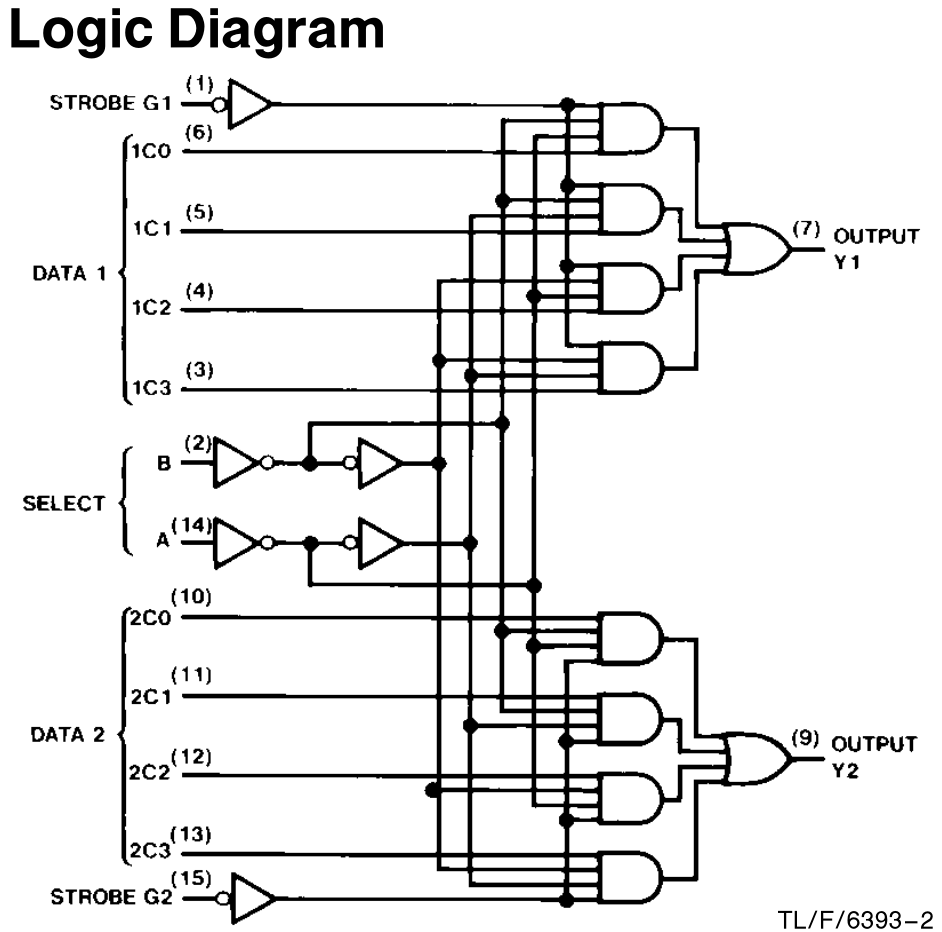
\includegraphics[width=.4\linewidth]{74LS153a.png}
	\caption{74LS153逻辑图}
	\label{fig:74LS153逻辑图}
\end{figure}

\begin{figure}[htbp]
	\centering
	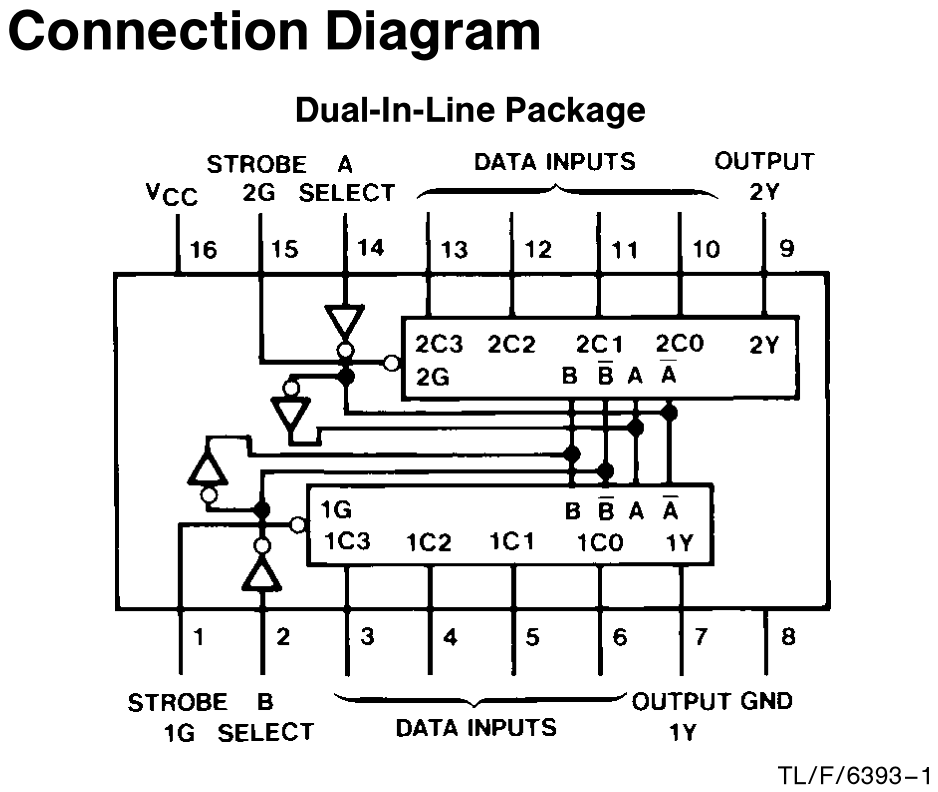
\includegraphics[width=.4\linewidth]{74LS153.png}
	\caption{74LS153引脚图}
	\label{fig:74LS153引脚图}
\end{figure}

\newpage
\section{实验步骤及结果}%
\label{sec:实验步骤及结果\arabic{chapter}}

\subsection{与非门和异或门设计全加器}%
\label{sub:与非门和异或门设计全加器}

确定全加器的输入、输出变量,并画出真值表。

依照真值表\ref{tab:全加器真值表},写出各输出变量的逻辑功能表达式并利用逻辑代数或卡诺图\ref{tab:全加器卡诺图}化简逻辑功能表达式\ref{eq:11}和\ref{eq:11a}。

\begin{table}[htbp]
	\centering
	\caption{全加器卡诺图}
	\label{tab:全加器卡诺图}
	\begin{subtable}[htbp]{.45\linewidth}
		\centering
		\caption{$C_i$}
		\label{tab:C}
		\stepcounter{subtable}
		\begin{tabu}to\linewidth{@{}X[c,3.5]@{}|X[c]X[c]X[c]X[c]@{}}
			$(A_iB_iC_{i-1})_{(2)}$& $(00)_{(2)}$ & $(01)_{(2)}$ & $(11)_{(2)}$ & $(10)_{(2)}$ \\
			\hline
			$0$ & $0$ & $0$ & $1$ & $0$ \\
			$1$ & $0$ & $1$ & $1$ & $1$ \\
		\end{tabu}
	\end{subtable}
	\quad
	\begin{subtable}[htbp]{.45\linewidth}
		\centering
		\caption{$S_i$}
		\label{tab:S}
		\begin{tabu}to\linewidth{@{}X[c,3.5]@{}|X[c]X[c]X[c]X[c]@{}}
			$(A_iB_iC_{i-1})_{(2)}$& $(00)_{(2)}$ & $(01)_{(2)}$ & $(11)_{(2)}$ & $(10)_{(2)}$ \\
			\hline
			$0$ & $0$ & $1$ & $0$ & $1$ \\
			$1$ & $1$ & $0$ & $1$ & $0$ \\
		\end{tabu}
	\end{subtable}
\end{table}

\begin{align}
	\label{eq:11}
	S_i&=A_i\otimes B_i \otimes C_{i-1}
	\\
	\label{eq:11a}
	C_i&=(A_i\otimes B_i)C_{i-1}+A_iB_i
\end{align}

变化表达式,采用与非门和异或门实现公式\ref{eq:11b}和\ref{eq:11c}:

\begin{align}
	\label{eq:11b}
	S_i&=A_i\otimes B_i \otimes C_{i-1}
	\\
	\label{eq:11c}
	C_i&=\overline{\overline{(A_i\otimes B_i)C_{i-1}}~\overline{A_iB_i}}
\end{align}

根据化简的输出逻辑表达式搭建电路\ref{fig:11}(开关当做输入信号,左掷为低电平,右掷为高电平,ChA-ChD 接到输出端可以观察输出信号)。8位开关的7、6、5位代表$(A_iB_iC_{i-1})_{(2)}$,红色的\textcolor{red}{ChA}、蓝色的\textcolor{blue}{ChB}代表$(C_iS_i)_{(2)}$。

\newcommand{\mypng}[3]{
	\begin{subfigure}[htbp]{.45\linewidth}
		\centering
		\begin{overpic}[width=\linewidth]{#1.png}
			\put(-.5,0){
				\includegraphics[width=\linewidth]{#3.eps}
			}
		\end{overpic}
		\caption{$#2$}
		\label{fig:#1}
	\end{subfigure}
}
\begin{figure}[htbp]
	\centering
	\mypng{11000}{(A_iB_iC_{i-1})_{(2)}=000\Rightarrow(C_iS_i)_{(2)}=00}{11}
	\quad
	\mypng{11001}{(A_iB_iC_{i-1})_{(2)}=001\Rightarrow(C_iS_i)_{(2)}=01}{11}

	\mypng{11010}{(A_iB_iC_{i-1})_{(2)}=010\Rightarrow(C_iS_i)_{(2)}=01}{11}
	\quad
	\mypng{11011}{(A_iB_iC_{i-1})_{(2)}=011\Rightarrow(C_iS_i)_{(2)}=10}{11}

	\mypng{11100}{(A_iB_iC_{i-1})_{(2)}=100\Rightarrow(C_iS_i)_{(2)}=01}{11}
	\quad
	\mypng{11101}{(A_iB_iC_{i-1})_{(2)}=101\Rightarrow(C_iS_i)_{(2)}=10}{11}

	\mypng{11110}{(A_iB_iC_{i-1})_{(2)}=110\Rightarrow(C_iS_i)_{(2)}=10}{11}
	\quad
	\mypng{11111}{(A_iB_iC_{i-1})_{(2)}=111\Rightarrow(C_iS_i)_{(2)}=11}{11}
	\caption{与非门和异或门设计全加器}
	\label{fig:11}
\end{figure}

\newpage
\subsection{与非门设计组合逻辑电路}%
\label{sub:与非门设计组合逻辑电路}

用与非门设计组合逻辑电路,其功能示意图如图\ref{fig:要求}所示:
确定输入、输出变量并画出真值表\ref{tab:组合逻辑电路}。

\begin{table}[htbp]
	\centering
	\caption{组合逻辑电路}
	\label{tab:组合逻辑电路}
	\begin{longtabu}to.5\linewidth{@{}*3{X[c]}|*1{X[C]}@{}}
		\toprule
		\multicolumn{3}{c|}{输入}   & 输出    \\ \midrule
		$A$ & $S_1$ & $S_0$ & $Z$ \\ \midrule
		0     & 0       & 0       & 0     \\
		0     & 0       & 1       & 0     \\
		0     & 1       & 0       & 0     \\
		0     & 1       & 1       & 1     \\
		1     & 0       & 0       & 1     \\
		1     & 0       & 1       & 0     \\
		1     & 1       & 0       & 1     \\
		1     & 1       & 1       & 1     \\ \bottomrule
	\end{longtabu}
\end{table}

写出输出变量的逻辑表达式\ref{eq:12}。

\begin{align}
	\label{eq:12}
	Z=AS_0+\overline{A}S_1
\end{align}

利用卡诺图\ref{tab:组合逻辑电路卡诺图}或逻辑代数化简逻辑表达式\ref{eq:12a}。

\begin{table}[htbp]
	\centering
	\caption{组合逻辑电路卡诺图}
	\label{tab:组合逻辑电路卡诺图}
	\begin{longtabu}to.5\linewidth{@{}X[c,3.5]@{}|X[c]X[c]X[c]X[c]@{}}
		$(AS_1S_0)_{(2)}$& $(00)_{(2)}$ & $(01)_{(2)}$ & $(11)_{(2)}$ & $(10)_{(2)}$ \\
		\hline
		$0$ & $0$ & $0$ & $1$ & $0$ \\
		$1$ & $1$ & $0$ & $1$ & $1$ \\
	\end{longtabu}
\end{table}

\begin{align}
	\label{eq:12a}
	Z=\overline{\overline{AS_0}~\overline{\overline{AS_1}S_1}}
\end{align}

根据输出逻辑表达式完成电路\ref{fig:12}搭建。8位开关的7、6、5位代表$(AS_1S_0)_{(2)}$,红色的\textcolor{red}{ChA}代表$Z$。验证电路准确性并截图保存。

\begin{figure}[htbp]
	\centering
	\mypng{12000}{(AS_1S_0)_{(2)}=000\Rightarrow Z=0}{12}
	\quad
	\mypng{12001}{(AS_1S_0)_{(2)}=001\Rightarrow Z=A=0}{12}

	\mypng{12010}{(AS_1S_0)_{(2)}=010\Rightarrow Z=\overline{A}=1}{12}
	\quad
	\mypng{12011}{(AS_1S_0)_{(2)}=011\Rightarrow Z=1}{12}

	\mypng{12100}{(AS_1S_0)_{(2)}=100\Rightarrow Z=0}{12}
	\quad
	\mypng{12101}{(AS_1S_0)_{(2)}=101\Rightarrow Z=A=1}{12}

	\mypng{12110}{(AS_1S_0)_{(2)}=110\Rightarrow Z=\overline{A}=0}{12}
	\quad
	\mypng{12111}{(AS_1S_0)_{(2)}=111\Rightarrow Z=1}{12}
	\caption{与非门设计组合逻辑电路}
	\label{fig:12}
\end{figure}

\newpage
\subsection{双四选一数据选择器设计全加器}%
\label{sub:双四选一数据选择器设计全加器}

确定输入、输出变量并画出真值表\ref{tab:全加器真值表}。标准与非式如公式\ref{eq:13}和\ref{eq:13a}所示。先用非门、与门和或门搭建了双四选一数据选择器,再利用数据选择器设计全加器。

\begin{align}
	\label{eq:13}
	C_i&=0\overline{A_i}~\overline{B_i}+C_{i-1}\overline{A_i}B_i+C_{i-1}A_i\overline{B_i}+1A_iB_i
	\\
	\label{eq:13a}
	S_i&=C_{i-1}\overline{A_i}~\overline{B_i}+\overline{C_{i-1}}~\overline{A_i}B_i+\overline{C_{i-1}}A_i\overline{B_i}+C_{i-1}A_iB_i
\end{align}

如图\ref{fig:13}所示,8位开关的7、6、5位代表$(A_iB_iC_{i-1})_{(2)}$,1、0位代表常数$0,1$,红色的\textcolor{red}{ChA}、蓝色的\textcolor{blue}{ChB}代表$(C_iS_i)_{(2)}$。

\begin{figure}[htbp]
	\centering
	\mypng{13000}{(A_iB_iC_{i-1})_{(2)}=000\Rightarrow(C_iS_i)_{(2)}=00}{11}
	\quad
	\mypng{13001}{(A_iB_iC_{i-1})_{(2)}=001\Rightarrow(C_iS_i)_{(2)}=01}{11}

	\mypng{13010}{(A_iB_iC_{i-1})_{(2)}=010\Rightarrow(C_iS_i)_{(2)}=01}{11}
	\quad
	\mypng{13011}{(A_iB_iC_{i-1})_{(2)}=011\Rightarrow(C_iS_i)_{(2)}=10}{11}

	\mypng{13100}{(A_iB_iC_{i-1})_{(2)}=100\Rightarrow(C_iS_i)_{(2)}=01}{11}
	\quad
	\mypng{13101}{(A_iB_iC_{i-1})_{(2)}=101\Rightarrow(C_iS_i)_{(2)}=10}{11}

	\mypng{13110}{(A_iB_iC_{i-1})_{(2)}=110\Rightarrow(C_iS_i)_{(2)}=10}{11}
	\quad
	\mypng{13111}{(A_iB_iC_{i-1})_{(2)}=111\Rightarrow(C_iS_i)_{(2)}=11}{11}
	\caption{双四选一数据选择器设计全加器}
	\label{fig:13}
\end{figure}

\newpage
\section{实验思考}%
\label{sec:实验思考\arabic{chapter}}

因为网络的原因实验预习报告中实验步骤的第三部分用双选一数据选择器设计全加器没有加载出来,在不知道实验平台上有已经搭好的双四选一数据选择器的情况下自己利用提供的模块重新搭了一个,布线有点乱,但结果是正确的。

\chapter{触发器设计及应用}%
\label{cha:触发器设计及应用\arabic{chapter}}

\section{实验目的}%
\label{sec:实验目的\arabic{chapter}}

\begin{enumerate}
	\item 熟悉触发器的基本逻辑功能;
	\item 掌握用触发器进行时序电路设计的一般方法;
	\item 理解和掌握触发器典型应用的工作原理及测试方法。
\end{enumerate}

\section{实验内容}%
\label{sec:实验内容\arabic{chapter}}

用触发器设计实现分频器电路与计时器电路。

\begin{enumerate}
	\item\label{it:1}按照表\ref{tab:D触发器逻辑功能表}给出的内容,逐项测试D触发器的逻辑功能并完成该表格:
	\item\label{it:2}用D触发器设计实现四分频电路(异步),观察并记录波形:
	\item\label{it:3}按照表\ref{tab:JK触发器逻辑功能表}给出的内容,逐项测试JK触发器的逻辑功能并完成该表格:
	\item\label{it:4}用JK触发器设计实现四分频电路(异步),观察并记录波形:
	\item\label{it:5}用JK触发器设计实现模五计数器电路(同步)。模五计数器状态转换关系如表\ref{tab:}所示。
\end{enumerate}

\begin{enumerate}
	\item 实验内容\ref{it:1}、\ref{it:3}测试后完成表格;
	\item 实验内容\ref{it:2}、\ref{it:4}、\ref{it:5}测试后保存实验电路,井将时钟及各触发器输出端信号结果截屏保存;
	\item 对实验\ref{it:4}与实验\ref{it:5}的时序信号进行截图对比,说明异步与同步时序电路的区别。
\end{enumerate}

\section{实验原理及相关设计}%
\label{sec:实验原理及相关设计\arabic{chapter}}

\subsection{D触发器}%
\label{sub:D触发器}

图\ref{fig:74LS153逻辑图}和图\ref{fig:74LS75引脚图}为D触发器逻辑图和内部结构图。触发器电路采用了维持阻塞结构,使它具有可靠性高和抗干扰能力强等忧点。触发器有异步置“0”、置“1”端,$\overline{R_D}$与$\overline{S_D}$低电平有效。D数据输入端、CP时钟输入端为上升沿触发。Q原态输出端,$\overline{Q}$反态输出端。逻辑功能表如表\ref{tab:D触发器逻辑功能表},图\ref{fig:D触发器传输方式}和\ref{fig:D触发器状态转换图}为D触发器传输方式与状态转换图。

\begin{figure}[htbp]
	\centering
	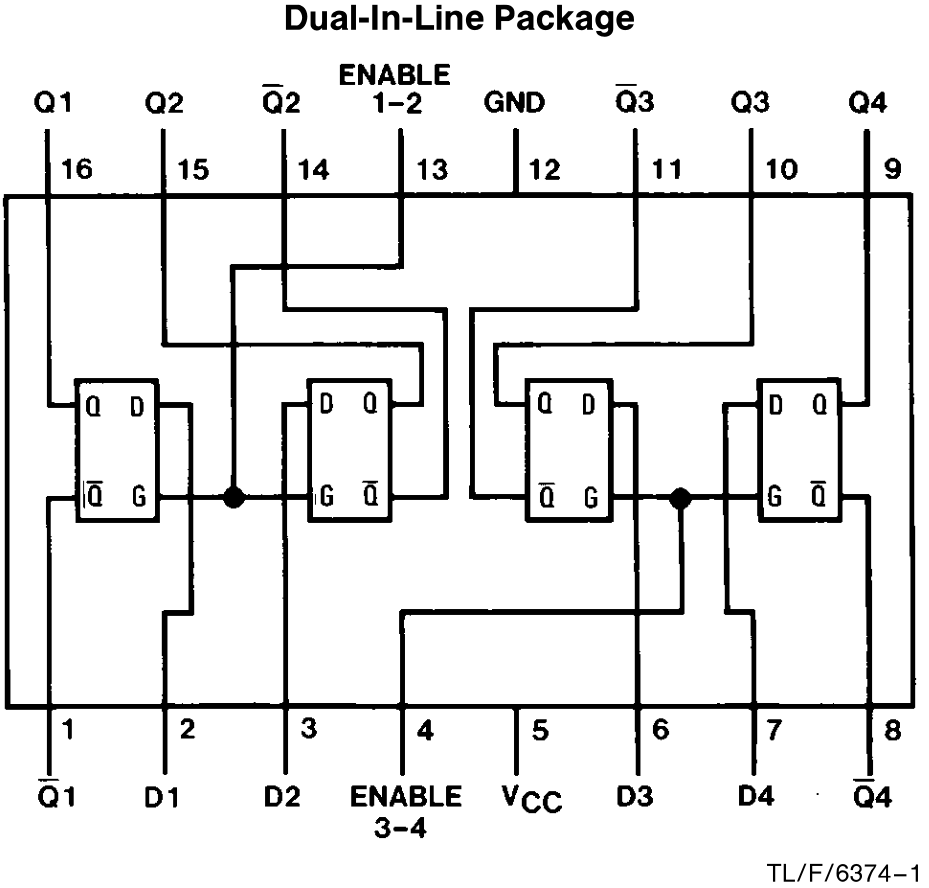
\includegraphics[width=.5\linewidth]{74LS75001.png}
	\caption{74LS75逻辑图}
	\label{fig:74LS75逻辑图}
\end{figure}

\begin{figure}[htbp]
	\centering
	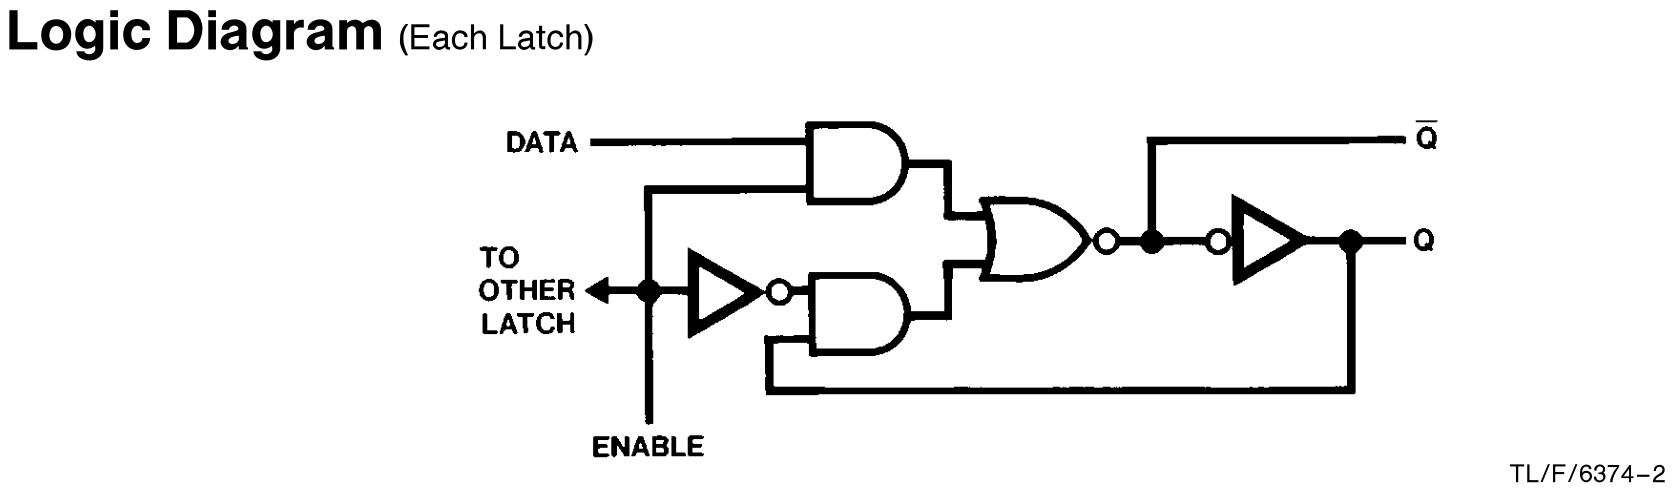
\includegraphics[width=.8\linewidth]{74LS75002.png}
	\caption{74LS75引脚图}
	\label{fig:74LS75引脚图}
\end{figure}

\begin{figure}[htbp]
	\centering
	\begin{subfigure}[htbp]{.45\linewidth}
		\centering
		% \usepackage[usenames,dvipsnames]{pstricks}
% \usepackage{epsfig}
% \usepackage{pst-grad} % For gradients
% \usepackage{pst-plot} % For axes
% \usepackage[space]{grffile} % For spaces in paths
% \usepackage{etoolbox} % For spaces in paths
% \makeatletter % For spaces in paths
% \patchcmd\Gread@eps{\@inputcheck#1 }{\@inputcheck"#1"\relax}{}{}
% \makeatother
% 
\psscalebox{1.0 1.0} % Change this value to rescale the drawing.
{
\begin{pspicture}(0,-2.2222223)(6.6666665,2.2222223)
\psframe[linecolor=black, linewidth=0.04, dimen=outer](4.888889,2.2222223)(1.7777778,-2.2222223)
\psline[linecolor=black, linewidth=0.04](1.7777778,1.3333334)(0.0,1.3333334)
\psline[linecolor=black, linewidth=0.04](1.7777778,0.0)(0.0,0.0)
\psline[linecolor=black, linewidth=0.04](4.888889,1.3333334)(6.6666665,1.3333334)(6.6666665,1.3333334)
\psline[linecolor=black, linewidth=0.04](4.888889,-1.3333334)(6.6666665,-1.3333334)
\rput[bl](2.2222223,1.3333334){\(D\)}
\rput[bl](2.2222223,0.0){CP}
\rput[bl](4.0,1.3333334){\(Q^n\)}
\rput[bl](4.0,-1.3333334){\(\overline{Q^n}\)}
\end{pspicture}
}


		\caption{D触发器传输方式}
		\label{fig:D触发器传输方式}
	\end{subfigure}
	\quad
	\begin{subfigure}[htbp]{.45\linewidth}
		\centering
		% Graphic for TeX using PGF
% Title: D:\User\Documents\Individual\Coursewares\Electronics\DigitalAndAnalog\0450\src\21.dia
% Creator: Dia v0.97.2
% CreationDate: Sun Apr 14 01:37:23 2019
% For: Wu Zhenyu
% \usepackage{tikz}
% The following commands are not supported in PSTricks at present
% We define them conditionally, so when they are implemented,
% this pgf file will use them.
\ifx\du\undefined
	\newlength{\du}
\fi
\setlength{\du}{10\unitlength}
\begin{tikzpicture}
	\pgftransformxscale{1.000000}
	\pgftransformyscale{-1.000000}
	\definecolor{dialinecolor}{rgb}{0.000000, 0.000000, 0.000000}
	\pgfsetstrokecolor{dialinecolor}
	\definecolor{dialinecolor}{rgb}{1.000000, 1.000000, 1.000000}
	\pgfsetfillcolor{dialinecolor}
	\definecolor{dialinecolor}{rgb}{1.000000, 1.000000, 1.000000}
	\pgfsetfillcolor{dialinecolor}
	\pgfpathellipse{\pgfpoint{22.771664\du}{15.674982\du}}{\pgfpoint{2.028364\du}{0\du}}{\pgfpoint{0\du}{2.001682\du}}
	\pgfusepath{fill}
	\pgfsetlinewidth{0.100000\du}
	\pgfsetdash{}{0pt}
	\pgfsetdash{}{0pt}
	\pgfsetmiterjoin
	\definecolor{dialinecolor}{rgb}{0.000000, 0.000000, 0.000000}
	\pgfsetstrokecolor{dialinecolor}
	\pgfpathellipse{\pgfpoint{22.771664\du}{15.674982\du}}{\pgfpoint{2.028364\du}{0\du}}{\pgfpoint{0\du}{2.001682\du}}
	\pgfusepath{stroke}
	% setfont left to latex
	\definecolor{dialinecolor}{rgb}{0.000000, 0.000000, 0.000000}
	\pgfsetstrokecolor{dialinecolor}
	\node at (22.771664\du,15.869982\du){0};
	\definecolor{dialinecolor}{rgb}{1.000000, 1.000000, 1.000000}
	\pgfsetfillcolor{dialinecolor}
	\pgfpathellipse{\pgfpoint{31.403364\du}{15.674982\du}}{\pgfpoint{2.028364\du}{0\du}}{\pgfpoint{0\du}{2.001682\du}}
	\pgfusepath{fill}
	\pgfsetlinewidth{0.100000\du}
	\pgfsetdash{}{0pt}
	\pgfsetdash{}{0pt}
	\pgfsetmiterjoin
	\definecolor{dialinecolor}{rgb}{0.000000, 0.000000, 0.000000}
	\pgfsetstrokecolor{dialinecolor}
	\pgfpathellipse{\pgfpoint{31.403364\du}{15.674982\du}}{\pgfpoint{2.028364\du}{0\du}}{\pgfpoint{0\du}{2.001682\du}}
	\pgfusepath{stroke}
	% setfont left to latex
	\definecolor{dialinecolor}{rgb}{0.000000, 0.000000, 0.000000}
	\pgfsetstrokecolor{dialinecolor}
	\node at (31.403364\du,15.869982\du){1};
	\pgfsetlinewidth{0.100000\du}
	\pgfsetdash{}{0pt}
	\pgfsetdash{}{0pt}
	\pgfsetmiterjoin
	\pgfsetbuttcap
	{
		\definecolor{dialinecolor}{rgb}{0.000000, 0.000000, 0.000000}
		\pgfsetfillcolor{dialinecolor}
		% was here!!!
		\pgfsetarrowsend{stealth}
		\definecolor{dialinecolor}{rgb}{0.000000, 0.000000, 0.000000}
		\pgfsetstrokecolor{dialinecolor}
		\pgfpathmoveto{\pgfpoint{24.750000\du}{14.000000\du}}
		\pgfpathcurveto{\pgfpoint{26.450000\du}{12.000000\du}}{\pgfpoint{27.700000\du}{12.200000\du}}{\pgfpoint{29.450000\du}{14.250000\du}}
		\pgfusepath{stroke}
	}
	\pgfsetlinewidth{0.100000\du}
	\pgfsetdash{}{0pt}
	\pgfsetdash{}{0pt}
	\pgfsetmiterjoin
	\pgfsetbuttcap
	{
		\definecolor{dialinecolor}{rgb}{0.000000, 0.000000, 0.000000}
		\pgfsetfillcolor{dialinecolor}
		% was here!!!
		\pgfsetarrowsend{stealth}
		\definecolor{dialinecolor}{rgb}{0.000000, 0.000000, 0.000000}
		\pgfsetstrokecolor{dialinecolor}
		\pgfpathmoveto{\pgfpoint{29.350000\du}{17.150000\du}}
		\pgfpathcurveto{\pgfpoint{28.100000\du}{18.950000\du}}{\pgfpoint{25.900000\du}{18.950000\du}}{\pgfpoint{24.700000\du}{17.200000\du}}
		\pgfusepath{stroke}
	}
	\pgfsetlinewidth{0.100000\du}
	\pgfsetdash{}{0pt}
	\pgfsetdash{}{0pt}
	\pgfsetmiterjoin
	\pgfsetbuttcap
	{
		\definecolor{dialinecolor}{rgb}{0.000000, 0.000000, 0.000000}
		\pgfsetfillcolor{dialinecolor}
		% was here!!!
		\pgfsetarrowsend{stealth}
		\definecolor{dialinecolor}{rgb}{0.000000, 0.000000, 0.000000}
		\pgfsetstrokecolor{dialinecolor}
		\pgfpathmoveto{\pgfpoint{20.700000\du}{17.900000\du}}
		\pgfpathcurveto{\pgfpoint{17.050000\du}{17.900000\du}}{\pgfpoint{17.500000\du}{14.100000\du}}{\pgfpoint{20.650000\du}{14.050000\du}}
		\pgfusepath{stroke}
	}
	\pgfsetlinewidth{0.100000\du}
	\pgfsetdash{}{0pt}
	\pgfsetdash{}{0pt}
	\pgfsetmiterjoin
	\pgfsetbuttcap
	{
		\definecolor{dialinecolor}{rgb}{0.000000, 0.000000, 0.000000}
		\pgfsetfillcolor{dialinecolor}
		% was here!!!
		\pgfsetarrowsend{stealth}
		\definecolor{dialinecolor}{rgb}{0.000000, 0.000000, 0.000000}
		\pgfsetstrokecolor{dialinecolor}
		\pgfpathmoveto{\pgfpoint{33.311000\du}{17.550300\du}}
		\pgfpathcurveto{\pgfpoint{37.200000\du}{17.500000\du}}{\pgfpoint{37.150000\du}{13.650000\du}}{\pgfpoint{33.261000\du}{13.700300\du}}
		\pgfusepath{stroke}
	}
	% setfont left to latex
	\definecolor{dialinecolor}{rgb}{0.000000, 0.000000, 0.000000}
	\pgfsetstrokecolor{dialinecolor}
	\node[anchor=west] at (16.450000\du,16.150000\du){D=0};
	% setfont left to latex
	\definecolor{dialinecolor}{rgb}{0.000000, 0.000000, 0.000000}
	\pgfsetstrokecolor{dialinecolor}
	\node[anchor=west] at (26.450000\du,19.350000\du){D=0};
	% setfont left to latex
	\definecolor{dialinecolor}{rgb}{0.000000, 0.000000, 0.000000}
	\pgfsetstrokecolor{dialinecolor}
	\node[anchor=west] at (26.400000\du,11.850000\du){D=1};
	% setfont left to latex
	\definecolor{dialinecolor}{rgb}{0.000000, 0.000000, 0.000000}
	\pgfsetstrokecolor{dialinecolor}
	\node[anchor=west] at (37.000000\du,15.700000\du){D=1};
\end{tikzpicture}

		\caption{D触发器状态转换图}
		\label{fig:D触发器状态转换图}
	\end{subfigure}
	\caption{D触发器传输方式和状态转换图}
	\label{fig:D触发器传输方式和状态转换图}
\end{figure}

\subsection{分频器}%
\label{sub:分频器}

分频器是将时钟高频率信号转变成低频率信号的一种转换器(n个脉冲周期使输出完成一个周期变化即为n次分频)。T触发器的表达式$Q^{n+1}=\overline{Q^n}$,工作状态实际为将输入的时钟频率降低一倍,即为二分频方式的分频器。计数器主要是计输入时钟的个数。

\subsection{JK触发器}%
\label{sub:JK触发器}
图\ref{fig:74HC76逻辑图}和\ref{fig:74HC76引脚图}为JK触发器逻辑图和引脚布局图。触发器有异步置“0”端、“1”端,$\overline{R_D}$与$\overline{S_D}$低电平有效,J、K数据输入端,CP时钟输入端,为下降沿触发。Q原态输出端,$\overline{Q}$反态输出端。逻辑功能表如表\ref{tab:JK触发器逻辑功能表}所示,图\ref{fig:JK触发器传输方式}和\ref{fig:JK触发器状态转换图}为JK触发器传输方式与状态转换图。

\begin{figure}[htbp]
	\centering
	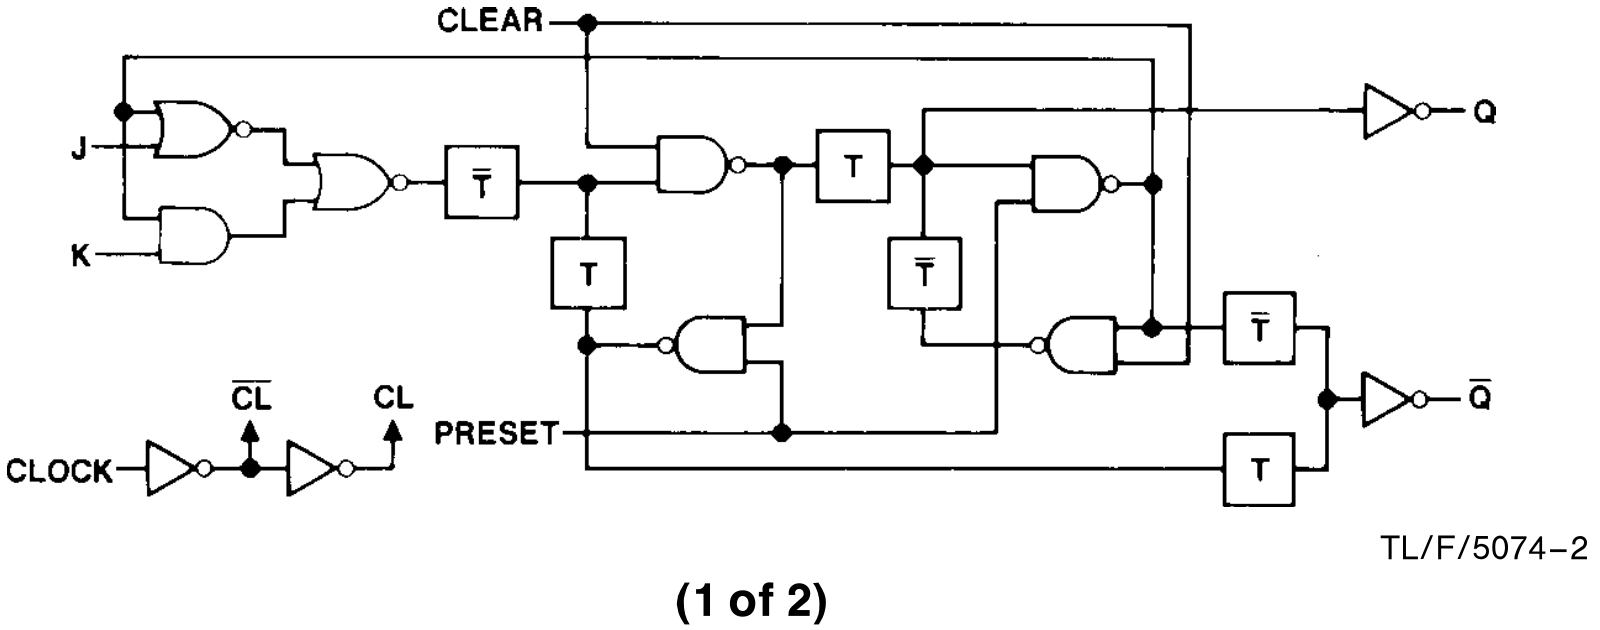
\includegraphics[width=.8\linewidth]{74HC76001.png}
	\caption{74HC76逻辑图}
	\label{fig:74HC76逻辑图}
\end{figure}

\begin{figure}[htbp]
	\centering
	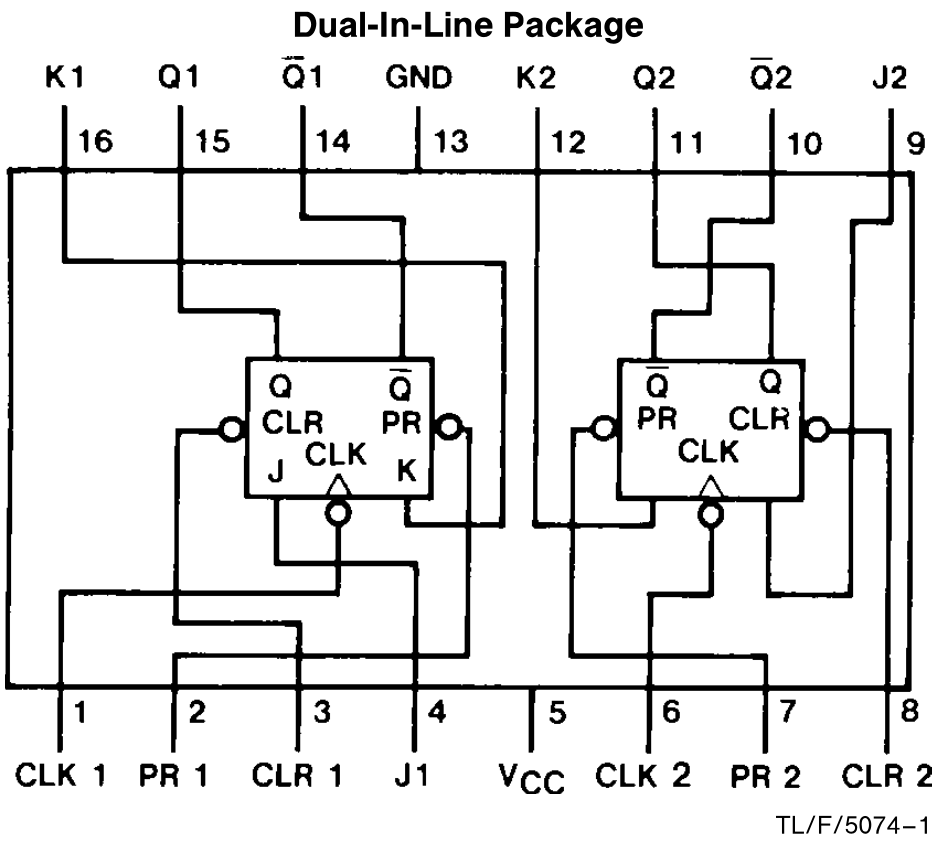
\includegraphics[width=.4\linewidth]{74HC76002.png}
	\caption{74HC76引脚图}
	\label{fig:74HC76引脚图}
\end{figure}

\begin{figure}[htbp]
	\centering
	\begin{subfigure}[htbp]{.45\linewidth}
		\centering
		% \usepackage[usenames,dvipsnames]{pstricks}
% \usepackage{epsfig}
% \usepackage{pst-grad} % For gradients
% \usepackage{pst-plot} % For axes
% \usepackage[space]{grffile} % For spaces in paths
% \usepackage{etoolbox} % For spaces in paths
% \makeatletter % For spaces in paths
% \patchcmd\Gread@eps{\@inputcheck#1 }{\@inputcheck"#1"\relax}{}{}
% \makeatother
% 
\psscalebox{1.0 1.0} % Change this value to rescale the drawing.
{
\begin{pspicture}(0,-2.2222223)(6.6666665,2.2222223)
\psframe[linecolor=black, linewidth=0.04, dimen=outer](4.888889,2.2222223)(1.7777778,-2.2222223)
\psline[linecolor=black, linewidth=0.04](1.7777778,1.3333334)(0.0,1.3333334)
\psline[linecolor=black, linewidth=0.04](1.7777778,0.0)(0.0,0.0)
\psline[linecolor=black, linewidth=0.04](1.7777778,-1.3333334)(0.0,-1.3333334)
\psline[linecolor=black, linewidth=0.04](4.888889,1.3333334)(6.6666665,1.3333334)(6.6666665,1.3333334)
\psline[linecolor=black, linewidth=0.04](4.888889,-1.3333334)(6.6666665,-1.3333334)
\rput[bl](2.2222223,1.3333334){\(J\)}
\rput[bl](2.2222223,0.0){CP}
\rput[bl](2.2222223,-1.3333334){\(K\)}
\rput[bl](4.0,1.3333334){\(Q^n\)}
\rput[bl](4.0,-1.3333334){\(\overline{Q^n}\)}
\end{pspicture}
}


		\caption{JK触发器传输方式}
		\label{fig:JK触发器传输方式}
	\end{subfigure}
	\quad
	\begin{subfigure}[htbp]{.45\linewidth}
		\centering
		% Graphic for TeX using PGF
% Title: D:\User\Documents\Individual\Coursewares\Electronics\DigitalAndAnalog\0450\src\23.dia
% Creator: Dia v0.97.2
% CreationDate: Sun Apr 14 01:36:06 2019
% For: Wu Zhenyu
% \usepackage{tikz}
% The following commands are not supported in PSTricks at present
% We define them conditionally, so when they are implemented,
% this pgf file will use them.
\ifx\du\undefined
	\newlength{\du}
\fi
\setlength{\du}{10\unitlength}
\begin{tikzpicture}
	\pgftransformxscale{1.000000}
	\pgftransformyscale{-1.000000}
	\definecolor{dialinecolor}{rgb}{0.000000, 0.000000, 0.000000}
	\pgfsetstrokecolor{dialinecolor}
	\definecolor{dialinecolor}{rgb}{1.000000, 1.000000, 1.000000}
	\pgfsetfillcolor{dialinecolor}
	\definecolor{dialinecolor}{rgb}{1.000000, 1.000000, 1.000000}
	\pgfsetfillcolor{dialinecolor}
	\pgfpathellipse{\pgfpoint{22.771664\du}{15.674982\du}}{\pgfpoint{2.028364\du}{0\du}}{\pgfpoint{0\du}{2.001682\du}}
	\pgfusepath{fill}
	\pgfsetlinewidth{0.100000\du}
	\pgfsetdash{}{0pt}
	\pgfsetdash{}{0pt}
	\pgfsetmiterjoin
	\definecolor{dialinecolor}{rgb}{0.000000, 0.000000, 0.000000}
	\pgfsetstrokecolor{dialinecolor}
	\pgfpathellipse{\pgfpoint{22.771664\du}{15.674982\du}}{\pgfpoint{2.028364\du}{0\du}}{\pgfpoint{0\du}{2.001682\du}}
	\pgfusepath{stroke}
	% setfont left to latex
	\definecolor{dialinecolor}{rgb}{0.000000, 0.000000, 0.000000}
	\pgfsetstrokecolor{dialinecolor}
	\node at (22.771664\du,15.869982\du){0};
	\definecolor{dialinecolor}{rgb}{1.000000, 1.000000, 1.000000}
	\pgfsetfillcolor{dialinecolor}
	\pgfpathellipse{\pgfpoint{31.403364\du}{15.674982\du}}{\pgfpoint{2.028364\du}{0\du}}{\pgfpoint{0\du}{2.001682\du}}
	\pgfusepath{fill}
	\pgfsetlinewidth{0.100000\du}
	\pgfsetdash{}{0pt}
	\pgfsetdash{}{0pt}
	\pgfsetmiterjoin
	\definecolor{dialinecolor}{rgb}{0.000000, 0.000000, 0.000000}
	\pgfsetstrokecolor{dialinecolor}
	\pgfpathellipse{\pgfpoint{31.403364\du}{15.674982\du}}{\pgfpoint{2.028364\du}{0\du}}{\pgfpoint{0\du}{2.001682\du}}
	\pgfusepath{stroke}
	% setfont left to latex
	\definecolor{dialinecolor}{rgb}{0.000000, 0.000000, 0.000000}
	\pgfsetstrokecolor{dialinecolor}
	\node at (31.403364\du,15.869982\du){1};
	\pgfsetlinewidth{0.100000\du}
	\pgfsetdash{}{0pt}
	\pgfsetdash{}{0pt}
	\pgfsetmiterjoin
	\pgfsetbuttcap
	{
		\definecolor{dialinecolor}{rgb}{0.000000, 0.000000, 0.000000}
		\pgfsetfillcolor{dialinecolor}
		% was here!!!
		\pgfsetarrowsend{stealth}
		\definecolor{dialinecolor}{rgb}{0.000000, 0.000000, 0.000000}
		\pgfsetstrokecolor{dialinecolor}
		\pgfpathmoveto{\pgfpoint{24.750000\du}{14.000000\du}}
		\pgfpathcurveto{\pgfpoint{26.450000\du}{12.000000\du}}{\pgfpoint{27.700000\du}{12.200000\du}}{\pgfpoint{29.450000\du}{14.250000\du}}
		\pgfusepath{stroke}
	}
	\pgfsetlinewidth{0.100000\du}
	\pgfsetdash{}{0pt}
	\pgfsetdash{}{0pt}
	\pgfsetmiterjoin
	\pgfsetbuttcap
	{
		\definecolor{dialinecolor}{rgb}{0.000000, 0.000000, 0.000000}
		\pgfsetfillcolor{dialinecolor}
		% was here!!!
		\pgfsetarrowsend{stealth}
		\definecolor{dialinecolor}{rgb}{0.000000, 0.000000, 0.000000}
		\pgfsetstrokecolor{dialinecolor}
		\pgfpathmoveto{\pgfpoint{29.650000\du}{17.150000\du}}
		\pgfpathcurveto{\pgfpoint{28.206900\du}{19.234000\du}}{\pgfpoint{25.700000\du}{19.000000\du}}{\pgfpoint{24.900000\du}{17.000000\du}}
		\pgfusepath{stroke}
	}
	\pgfsetlinewidth{0.100000\du}
	\pgfsetdash{}{0pt}
	\pgfsetdash{}{0pt}
	\pgfsetmiterjoin
	\pgfsetbuttcap
	{
		\definecolor{dialinecolor}{rgb}{0.000000, 0.000000, 0.000000}
		\pgfsetfillcolor{dialinecolor}
		% was here!!!
		\pgfsetarrowsend{stealth}
		\definecolor{dialinecolor}{rgb}{0.000000, 0.000000, 0.000000}
		\pgfsetstrokecolor{dialinecolor}
		\pgfpathmoveto{\pgfpoint{20.700000\du}{17.900000\du}}
		\pgfpathcurveto{\pgfpoint{17.050000\du}{17.900000\du}}{\pgfpoint{17.500000\du}{14.100000\du}}{\pgfpoint{20.650000\du}{14.050000\du}}
		\pgfusepath{stroke}
	}
	\pgfsetlinewidth{0.100000\du}
	\pgfsetdash{}{0pt}
	\pgfsetdash{}{0pt}
	\pgfsetmiterjoin
	\pgfsetbuttcap
	{
		\definecolor{dialinecolor}{rgb}{0.000000, 0.000000, 0.000000}
		\pgfsetfillcolor{dialinecolor}
		% was here!!!
		\pgfsetarrowsend{stealth}
		\definecolor{dialinecolor}{rgb}{0.000000, 0.000000, 0.000000}
		\pgfsetstrokecolor{dialinecolor}
		\pgfpathmoveto{\pgfpoint{33.311000\du}{17.550300\du}}
		\pgfpathcurveto{\pgfpoint{37.200000\du}{17.500000\du}}{\pgfpoint{37.150000\du}{13.650000\du}}{\pgfpoint{33.261000\du}{13.700300\du}}
		\pgfusepath{stroke}
	}
	% setfont left to latex
	\definecolor{dialinecolor}{rgb}{0.000000, 0.000000, 0.000000}
	\pgfsetstrokecolor{dialinecolor}
	\node[anchor=west] at (17.950000\du,19.000000\du){J=0,K=x};
	% setfont left to latex
	\definecolor{dialinecolor}{rgb}{0.000000, 0.000000, 0.000000}
	\pgfsetstrokecolor{dialinecolor}
	\node[anchor=west] at (26.000000\du,19.600000\du){J=x,K=1};
	% setfont left to latex
	\definecolor{dialinecolor}{rgb}{0.000000, 0.000000, 0.000000}
	\pgfsetstrokecolor{dialinecolor}
	\node[anchor=west] at (25.975000\du,11.995000\du){J=1,K=x};
	% setfont left to latex
	\definecolor{dialinecolor}{rgb}{0.000000, 0.000000, 0.000000}
	\pgfsetstrokecolor{dialinecolor}
	\node[anchor=west] at (34.450000\du,18.645000\du){J=x,K=0};
\end{tikzpicture}

		\caption{JK触发器状态转换图}
		\label{fig:JK触发器状态转换图}
	\end{subfigure}
	\caption{JK触发器传输方式和状态转换图}
	\label{fig:JK触发器传输方式和状态转换图}
\end{figure}

\section{实验步骤及结果}%
\label{sec:实验步骤及结果\arabic{chapter}}

\subsection{测试D触发器逻辑功能}%
\label{sub:测试D触发器逻辑功能}

\begin{table}[htbp]
	\centering
	\caption{D触发器逻辑功能表}
	\label{tab:D触发器逻辑功能表}
	\small
	\begin{longtabu}to\linewidth{@{}X[c]|X[c]X[c]X[c]X[c]|X[c]X[c]@{}}
		\toprule
		功能 & \multicolumn{4}{c}{输入} & \multicolumn{2}{|c}{输出} \\
		\midrule
			 & CP & $ \overline{R_D} $ & $ \overline{S_D} $ & $D$ & $Q^{n+1}$ & $ \overline{Q^{n+1}} $\\
			 \midrule
		异步复位 & $x$ & 1 & 0 & $x$ & 0 & 1 \\
		异步置位 & $x$ & 0 & 1 & $x$ & 1 & 0 \\
		同步跟随 & $\uparrow$ & 1 & 1 & 0 & 0 & 1 \\
		同步跟随 & $\uparrow$ & 1 & 1 & 1 & 1 & 0 \\
		异步保持 & 0 & 1 & 1 & $x$ & \multicolumn{2}{c}{$Q^{n+1}=Q^n, \overline{Q^{n+1}}= \overline{Q^n}  $} \\
		无效 & $x$ & 0 & 0 & $x$ & \multicolumn{2}{c}{$Q^{n+1}=0, \overline{Q^{n+1}}=1 $} \\
		\bottomrule
	\end{longtabu}
\end{table}

\subsection{用D触发器实现异步4分频电路}%
\label{sub:用D触发器实现异步4分频电路}

D触发器设计成2分频电路实际是将D触发器设计成T'触发器。可得$D=\overline{Q_n}$。

\begin{figure}[htbp]
	\centering
	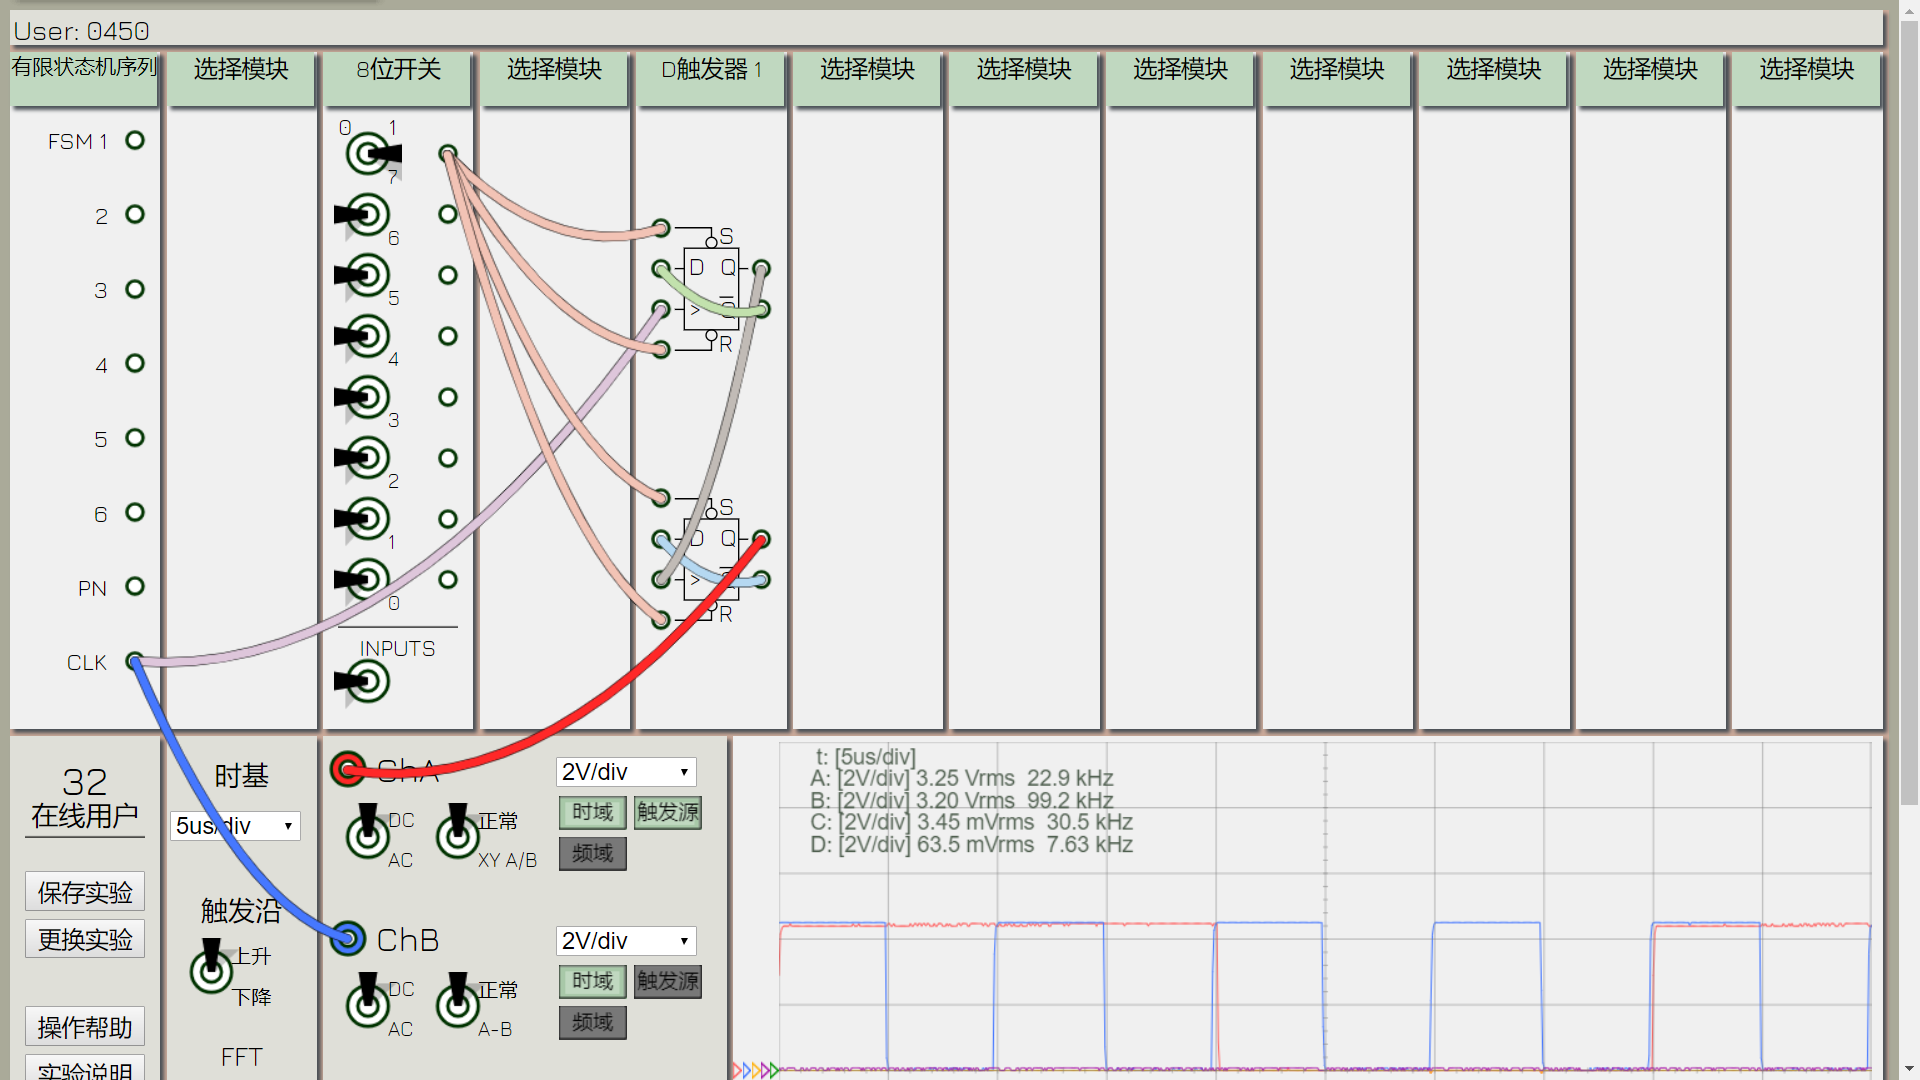
\includegraphics[width=.7\linewidth]{22.png}
	\caption{用D触发器实现异步4分频电路}
	\label{fig:用D触发器实现异步4分频电路}
\end{figure}

\newpage
\subsection{测试JK触发器逻辑功能}%
\label{sub:测试JK触发器逻辑功能}

\begin{table}[htbp]
	\centering
	\caption{JK触发器逻辑功能表}
	\label{tab:JK触发器逻辑功能表}
	\small
	\begin{longtabu}to\linewidth{@{}X[c]|X[c]X[c]X[c]X[c]X[c]|X[c]X[c]@{}}
		\toprule
		功能 & \multicolumn{5}{c}{输入} & \multicolumn{2}{|c}{输出} \\
		\midrule
			 & $ \overline{CP} $  & $ \overline{R_D}  $ & $ \overline{S_D}  $ & J & K & $ Q^{n+1} $ & $ \overline{Q^{n+1}}  $\\
			 \midrule
		异步复位 & $x$ & 0 & 1 & $x$ & $x$ & 0 & 1\\
		异步置位 & $x$ & 1 & 0 & $x$ & $x$ & 1 & 0\\
		异步保持 & $x$ & 1 & 1 & 0 & 0 & \multicolumn{2}{c}{$ Q^{n+1}=Q^n, \overline{Q^{n+1}} = \overline{Q^n}  $} \\
		同步复位 & $ \downarrow $ & 1 & 1 & 0 & 1 & 0 & 1\\
		同步置位 & $ \downarrow $ & 1 & 1 & 1 & 0 & 1 & 0\\
		同步反转 & $ \downarrow $ & 1 & 1 & 1 & 0 & $ \overline{Q^n} $ & $ Q^n $\\
		同步保持 & $ \downarrow $ & 1 & 1 & 1 & 1 & $ Q^n $ & $ \overline{Q^n} $ \\
		无效 & $x$ & 0 & 0 & $x$ & $x$ & \multicolumn{2}{c}{$ Q^{n+1}=0, \overline{Q^{n+1}}=1  $} \\
		\bottomrule
	\end{longtabu}
	\vspace{-2em}
\end{table}

\subsection{用JK触发器实现异步4分频电路}%
\label{sub:用JK触发器实现异步4分频电路}

JK触发器设计2分频电路实际是将JK触发器设计T'触发器。有$J=1,K=1$,也可用公式对比得到$Q^{n+1}=J\overline{Q^n}+\overline{K}Q^n$,设$J=K=T=1$,表达式为$Q^{n+1}=\overline{Q^n}$,即为T'触发器。

\begin{figure}[htbp]
	\centering
	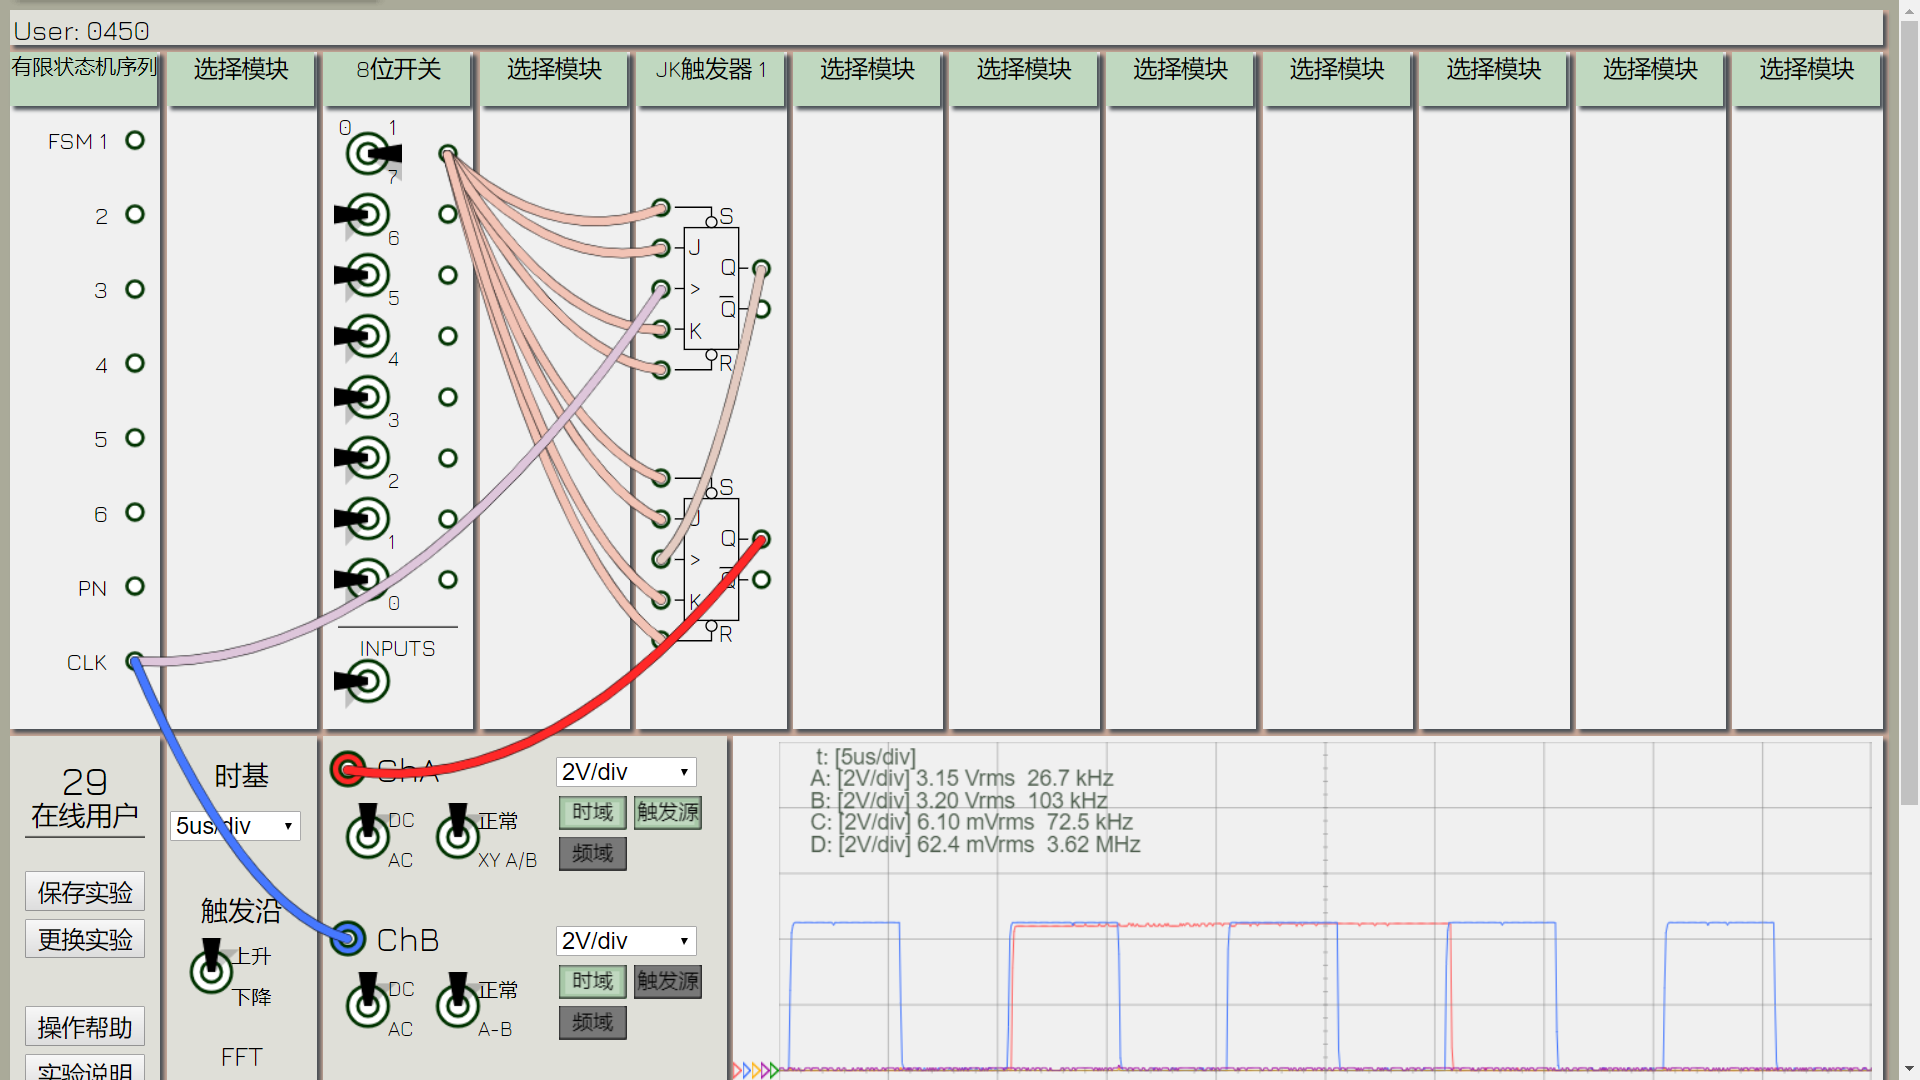
\includegraphics[width=.7\linewidth]{24.png}
	\caption{用JK触发器实现异步4分频电路}
	\label{fig:用JK触发器实现异步4分频电路}
\end{figure}

\newpage
\subsection{用JK触发器实现同步模5计数器}%
\label{sub:用JK触发器实现同步模5计数器}

\begin{enumerate}
	\item 填写状态转换真值表\ref{tab:同步模5计数器状态转换真值表及激励信号}及激励信号;

		\begin{table}[htbp]
			\centering
			\caption{同步模5计数器状态转换真值表及激励信号}
			\label{tab:同步模5计数器状态转换真值表及激励信号}
			\begin{longtabu}to\linewidth{@{}X[c]X[c]X[c]|X[c]X[c]X[c]|X[c]X[c]|X[c]X[c]|X[c]X[c]@{}}
				\toprule
				$ Q^n_2 $ & $ Q^n_1 $ & $ Q^n_0 $ & $ Q^{n+1}_2 $ & $ Q^{n+1}_1 $ & $ Q^{n+1}_0 $ & $ J_2 $ & $ K_2 $ & $ J_1 $ & $ K_1 $ & $ J_0 $ & $ K_0 $ \\
				\midrule
				0 & 0 & 0 & 0 & 0 & 1 & 0 & x & 0 & x & 1 & x\\
				0 & 0 & 1 & 0 & 1 & 0 & 0 & x & 1 & x & x & 1\\
				0 & 1 & 0 & 0 & 1 & 1 & 0 & x & x & 0 & 1 & x\\
				0 & 1 & 1 & 1 & 0 & 0 & 1 & x & x & 1 & x & 1\\
				1 & 0 & 0 & 0 & 0 & 0 & x & 1 & 0 & x & 0 & x\\
				x & x & x & x & x & x & x & x & x & x & x & x\\
				\bottomrule
			\end{longtabu}
		\end{table}

	\item 绘制$ J_i,K_i $卡诺图\ref{tab:同步模5计数器卡诺图},由卡诺图化简得到各激励方程\ref{eq:25};

		\begin{table}[htbp]
			\centering
			\caption{同步模5计数器卡诺图}
			\label{tab:同步模5计数器卡诺图}
			\begin{subtable}[htbp]{.45\linewidth}
				\centering
				\caption{$ J_2 $}
				\label{tab:J2}
				\begin{tabu}to\linewidth{@{}X[c,3.5]@{}|X[c]X[c]X[c]X[c]@{}}
					$(Q_2Q_1Q_0)_{(2)}$& $(00)_{(2)}$ & $(01)_{(2)}$ & $(11)_{(2)}$ & $(10)_{(2)}$ \\
					\hline
					$0$ & $0$ & $0$ & $1$ & $0$ \\
					$1$ & $x$ & $x$ & $x$ & $x$ \\
				\end{tabu}
			\end{subtable}
			\quad
			\begin{subtable}[htbp]{.45\linewidth}
				\centering
				\caption{$ K_2 $}
				\label{tab:K2}
				\begin{tabu}to\linewidth{@{}X[c,3.5]@{}|X[c]X[c]X[c]X[c]@{}}
					$(Q_2Q_1Q_0)_{(2)}$& $(00)_{(2)}$ & $(01)_{(2)}$ & $(11)_{(2)}$ & $(10)_{(2)}$ \\
					\hline
					$0$ & $x$ & $x$ & $x$ & $x$ \\
					$1$ & $1$ & $x$ & $x$ & $x$ \\
				\end{tabu}
			\end{subtable}

			\vspace{2em}
			\begin{subtable}[htbp]{.45\linewidth}
				\centering
				\caption{$ J_1 $}
				\label{tab:J1}
				\begin{tabu}to\linewidth{@{}X[c,3.5]@{}|X[c]X[c]X[c]X[c]@{}}
					$(Q_2Q_1Q_0)_{(2)}$& $(00)_{(2)}$ & $(01)_{(2)}$ & $(11)_{(2)}$ & $(10)_{(2)}$ \\
					\hline
					$0$ & $0$ & $1$ & $x$ & $x$ \\
					$1$ & $0$ & $x$ & $x$ & $x$ \\
				\end{tabu}
			\end{subtable}
			\quad
			\begin{subtable}[htbp]{.45\linewidth}
				\centering
				\caption{$ K_1 $}
				\label{tab:K1}
				\begin{tabu}to\linewidth{@{}X[c,3.5]@{}|X[c]X[c]X[c]X[c]@{}}
					$(Q_2Q_1Q_0)_{(2)}$& $(00)_{(2)}$ & $(01)_{(2)}$ & $(11)_{(2)}$ & $(10)_{(2)}$ \\
					\hline
					$0$ & $x$ & $x$ & $1$ & $0$ \\
					$1$ & $x$ & $x$ & $x$ & $x$ \\
				\end{tabu}
			\end{subtable}

			\vspace{2em}
			\begin{subtable}[htbp]{.45\linewidth}
				\centering
				\caption{$ J_0 $}
				\label{tab:J0}
				\begin{tabu}to\linewidth{@{}X[c,3.5]@{}|X[c]X[c]X[c]X[c]@{}}
					$(Q_2Q_1Q_0)_{(2)}$& $(00)_{(2)}$ & $(01)_{(2)}$ & $(11)_{(2)}$ & $(10)_{(2)}$ \\
					\hline
					$0$ & $1$ & $x$ & $1$ & $x$ \\
					$1$ & $x$ & $x$ & $x$ & $x$ \\
				\end{tabu}
			\end{subtable}
			\quad
			\begin{subtable}[htbp]{.45\linewidth}
				\centering
				\caption{$ K_0 $}
				\label{tab:K0}
				\begin{tabu}to\linewidth{@{}X[c,3.5]@{}|X[c]X[c]X[c]X[c]@{}}
					$(Q_2Q_1Q_0)_{(2)}$& $(00)_{(2)}$ & $(01)_{(2)}$ & $(11)_{(2)}$ & $(10)_{(2)}$ \\
					\hline
					$0$ & $x$ & $1$ & $1$ & $x$ \\
					$1$ & $x$ & $x$ & $x$ & $x$ \\
				\end{tabu}
			\end{subtable}
		\end{table}

		\newpage
		\begin{align}
			\label{eq:25}
			J_2&=Q^n_1Q^n_0\\
			K_2 & =1\\
			J_1 & =Q^n_0\\
			K_1 & =Q^n_0\\
			J_0 & =Q_0^n+ \overline{Q_1^n} \\
			K_0 & =1
		\end{align}

	\item 根据激励方程\ref{eq:25}连接并测试。
		\begin{figure}[htbp]
			\centering
			\begin{overpic}[width=\linewidth]{25.png}
				\put(-2,0){
					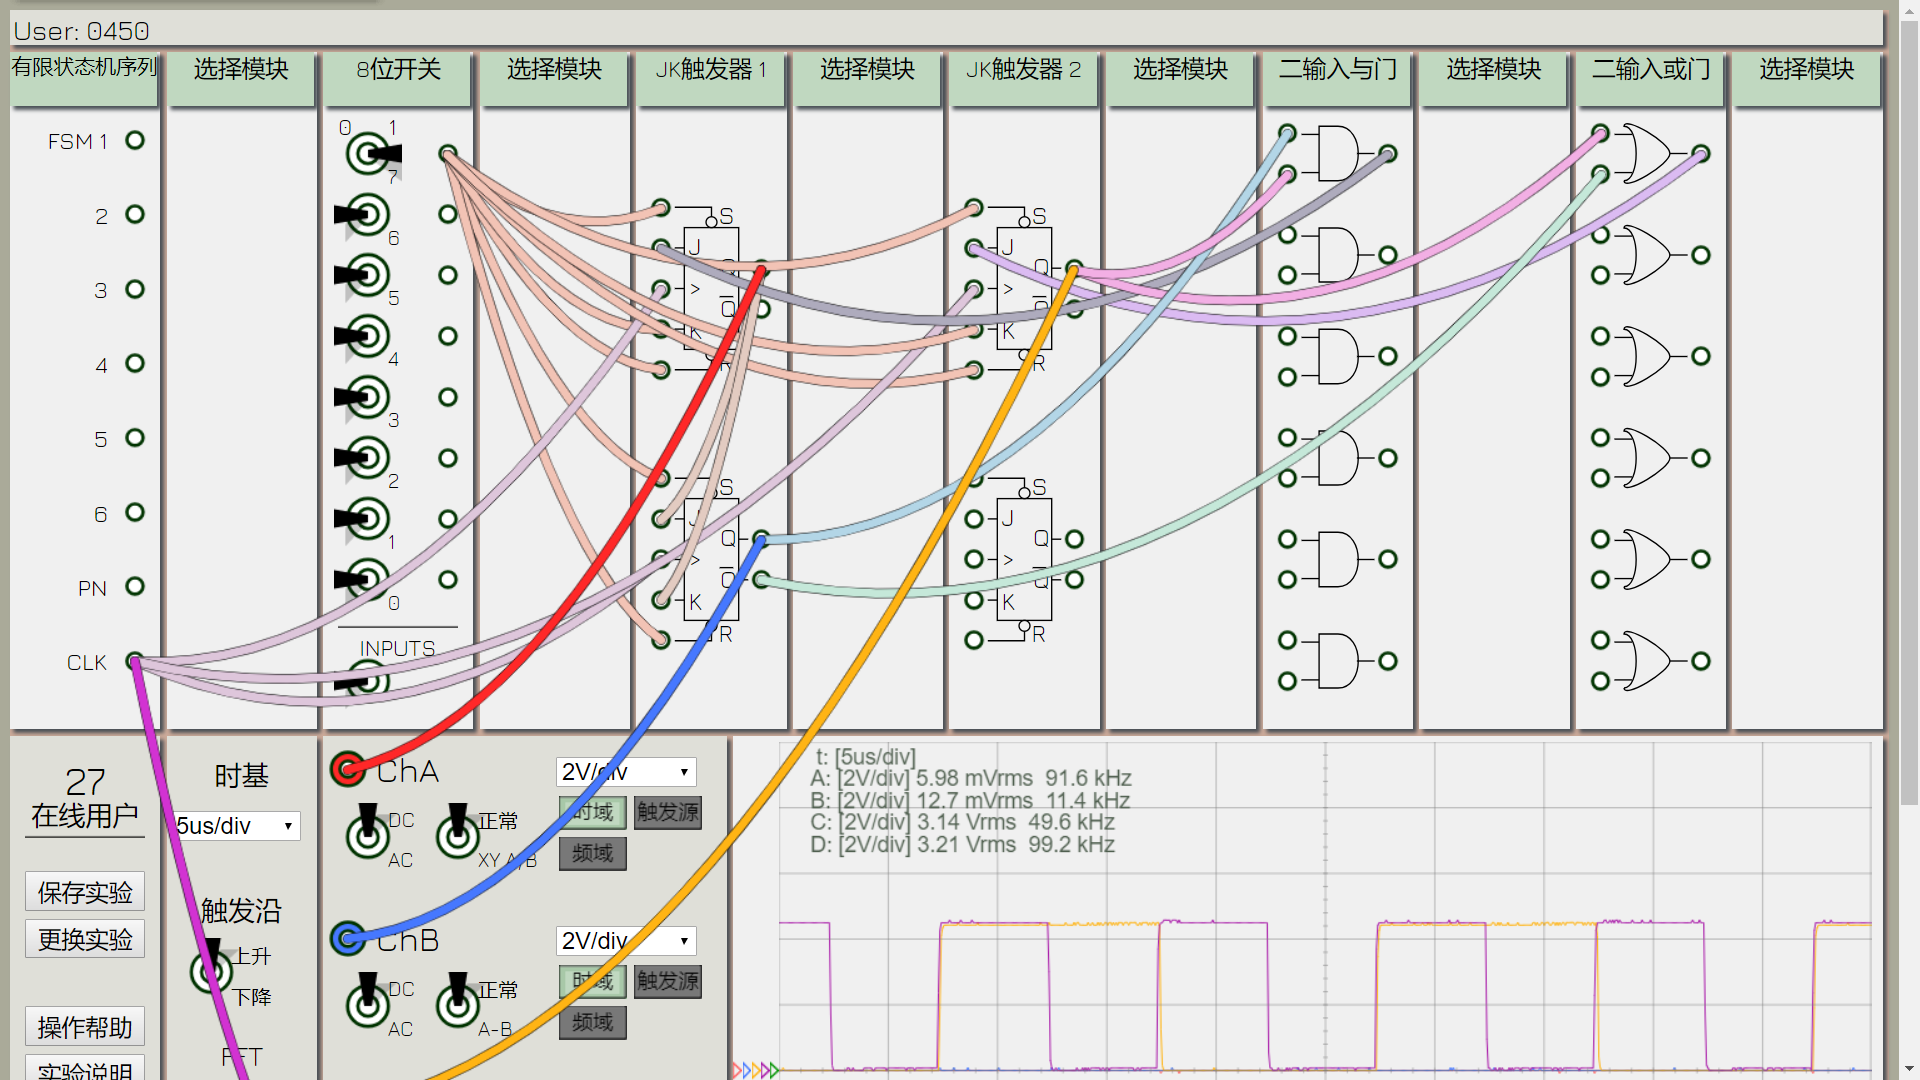
\includegraphics[width=\linewidth]{25.eps}
				}
			\end{overpic}
			\caption{用JK触发器实现同步模5计数器}
			\label{fig:用JK触发器实现同步模5计数器}
		\end{figure}
\end{enumerate}

\newpage
\section{实验思考}%
\label{sec:实验思考\arabic{chapter}}

值得注意的是当D触发器和JK触发器处于无效状态时结果并不是$ Q^n= \overline{Q^n}=1 $,而是$ Q^n=0, \overline{Q^n}=1 $。可能是仿真模块设计原因。

\begin{figure}[htbp]
	\vspace{-.5em}
	\centering
	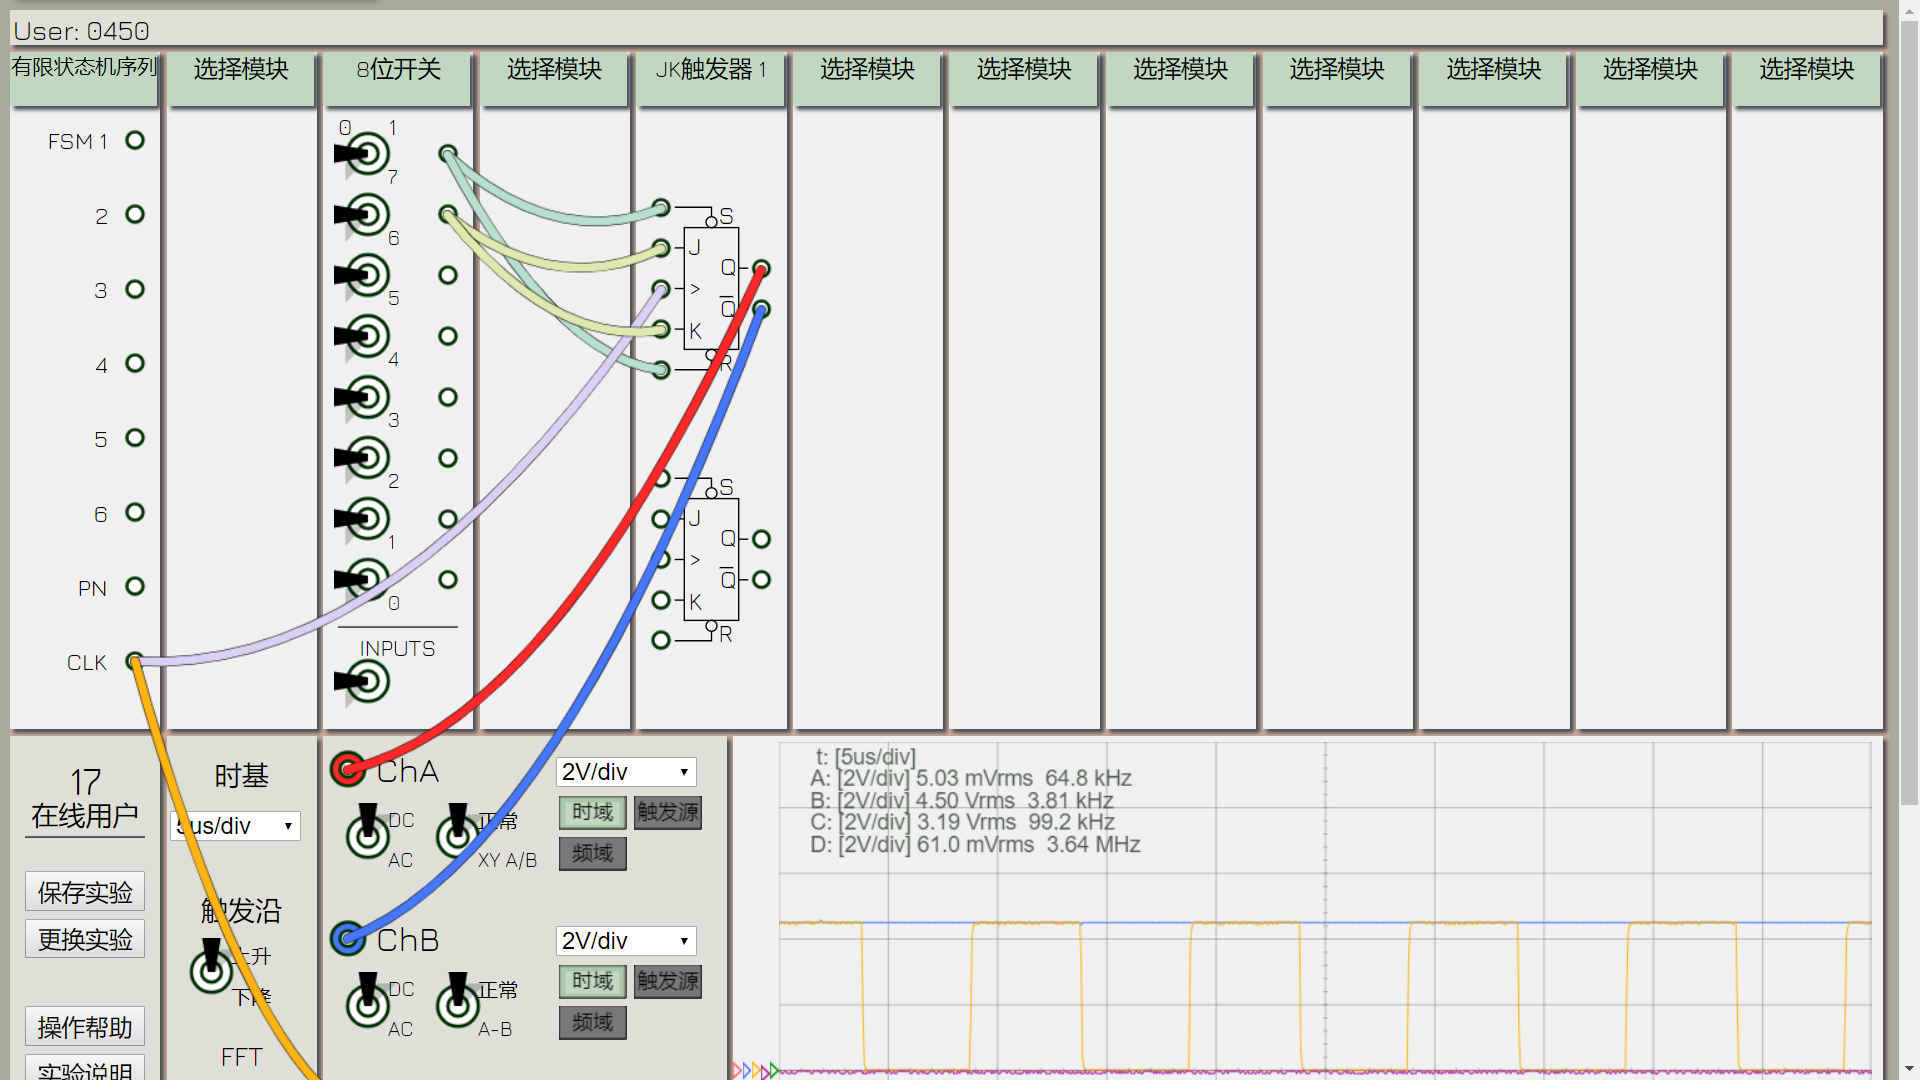
\includegraphics[width=.8\linewidth]{21.png}
	\caption{D触发器无效}
	\label{fig:D触发器无效}

	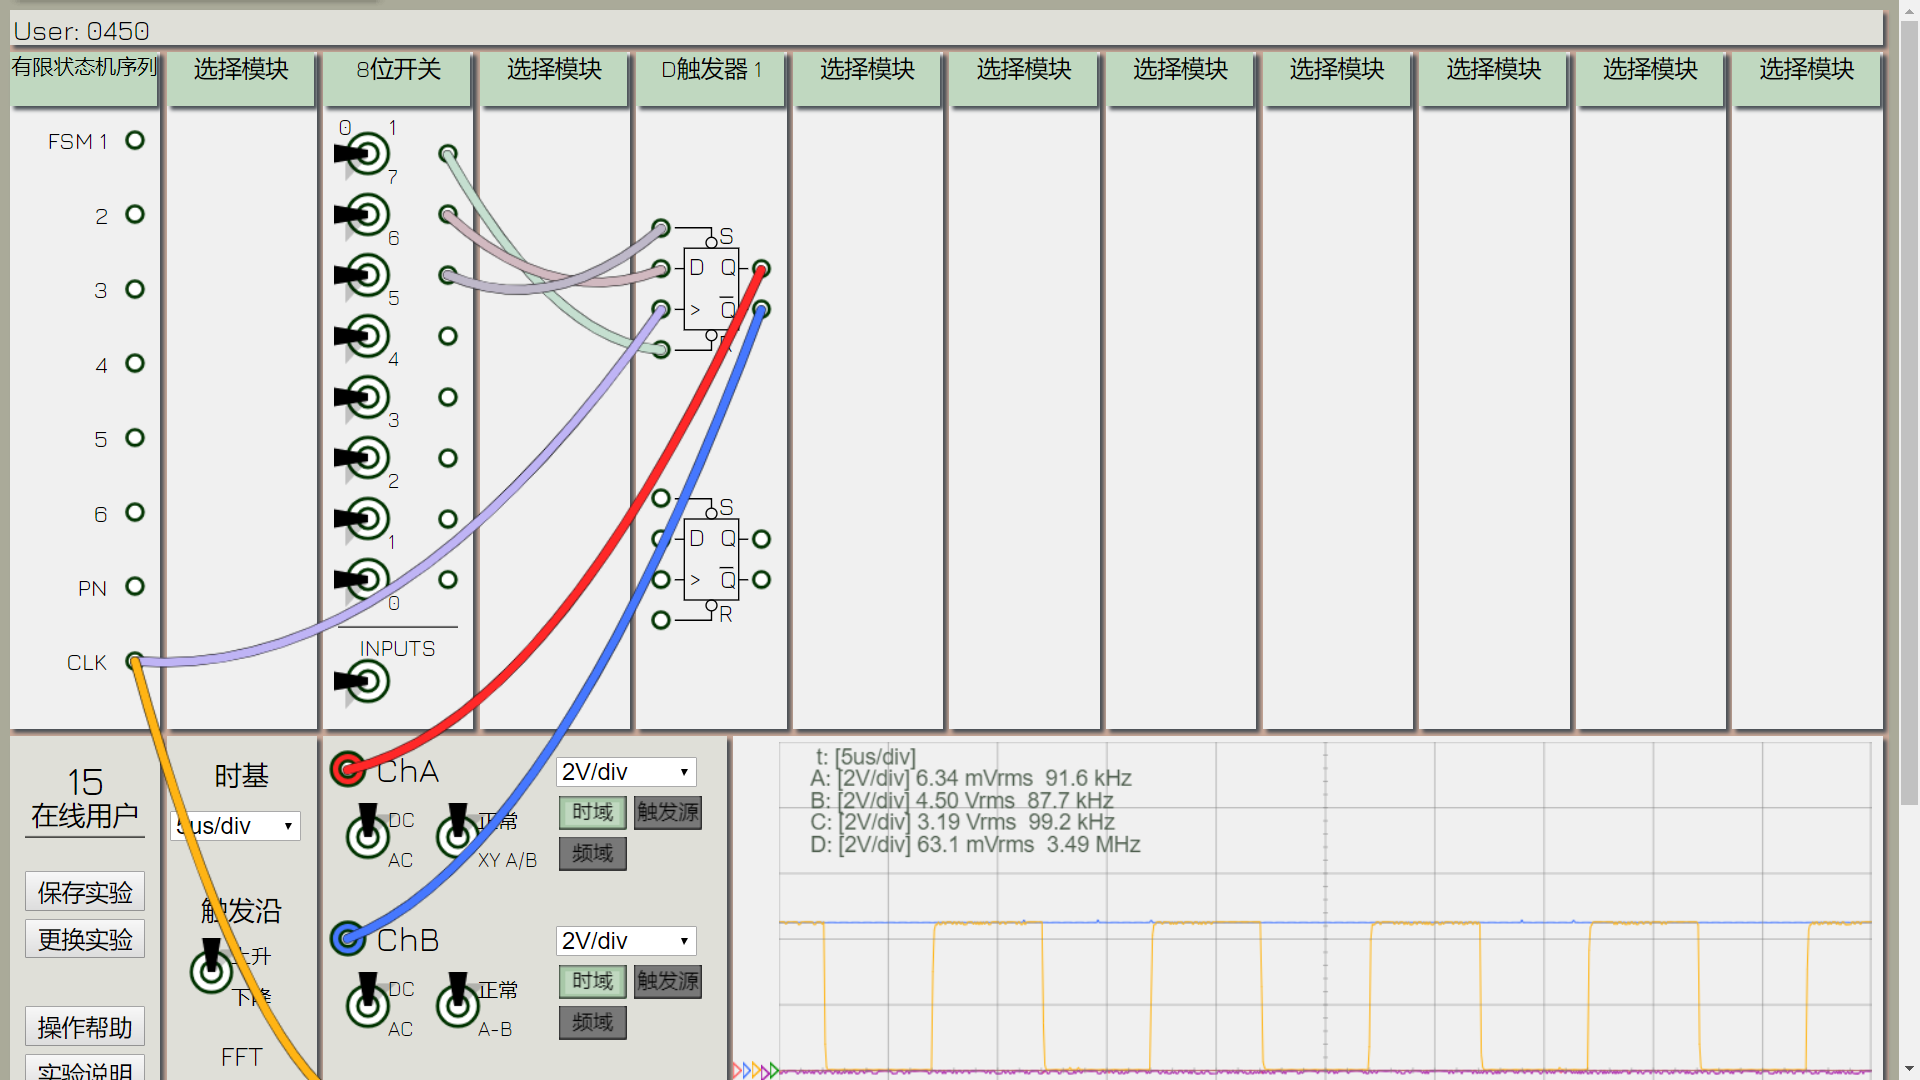
\includegraphics[width=.8\linewidth]{23.png}
	\caption{JK触发器无效}
	\label{fig:JK触发器无效}
\end{figure}

\chapter{任意进制计数器设计}%
\label{cha:任意进制计数器设计}

\section{实验目的}%
\label{sec:实验目的\arabic{chapter}}

掌握任意进制计数器的逻辑功能及其应用。

实现模十六内任意区间电路设计与十进制计数器工作波形绘制。

\section{实验内容}%
\label{sec:实验内容\arabic{chapter}}

\begin{enumerate}
	\item 按表\ref{tab:74LS161逻辑表}测试74LS161四位二进制计数器逻辑功能。
	\item \label{it:32}用74LS161四位二进制计数器设计完成$ 0..5\rightarrow A..D\rightarrow 0 $区间计数器。
	\item 按表\ref{tab:CD4518逻辑表}测试CD4518BCD码计数器逻辑功能。
	\item \label{it:34}绘制CD4518BCD码计数器工作波形(EN为时钟脉冲输入端)。
\end{enumerate}

实验报告要求如下:

\begin{enumerate}
	\item 要画出所使用的器件引脚排布图与逻辑功能表;
	\item 绘制实验内容\ref{it:32}的实验电路并阐述设计方法;
	\item 绘制实验内容\ref{it:34}的波形图;
	\item 格式与其他内容参考实验报告模版。
\end{enumerate}

\section{实验原理及相关设计}%
\label{sec:实验原理及相关设计\arabic{chapter}}

\subsection{74LS161四位二进制同步加法计数器}%
\label{sub:74LS161四位二进制同步加法计数器}

74LS161四位二进制同步加法计数器逻辑图如图\ref{fig:74LS161逻辑图}与引脚局部图如图\ref{fig:74LS161引脚图}。

\begin{figure}[htbp]
	\centering
	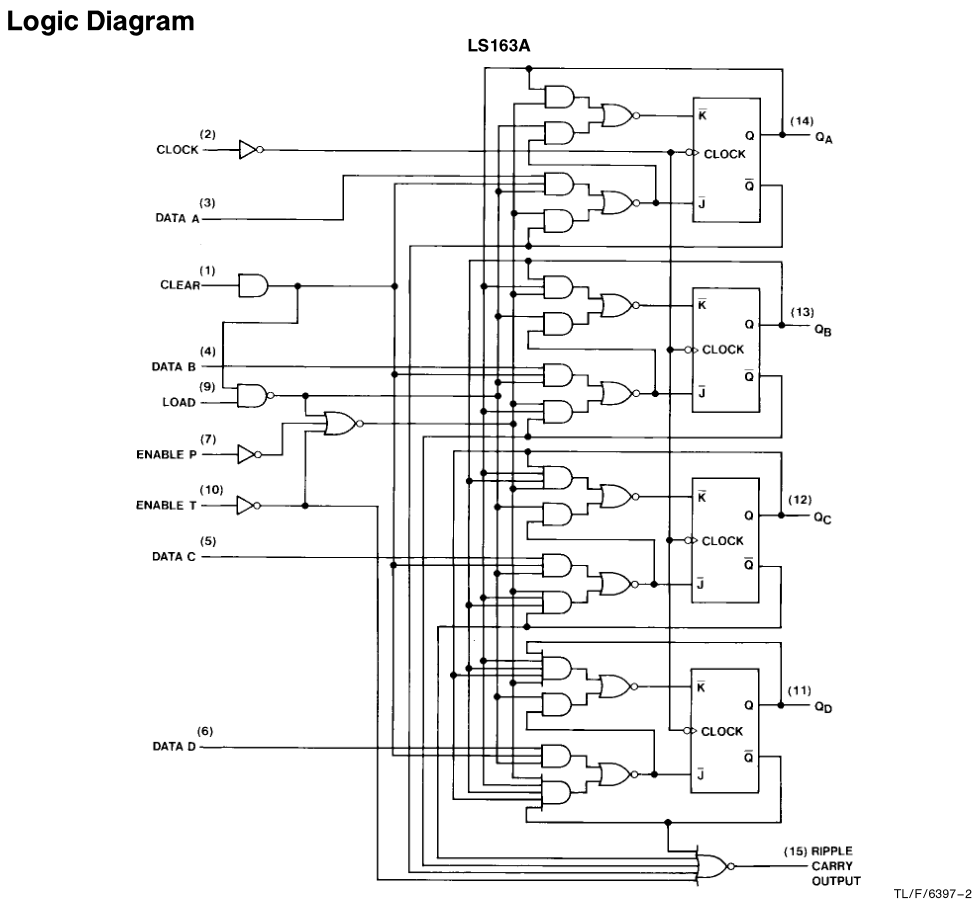
\includegraphics[width=.5\linewidth]{74LS161001.png}
	\caption{74LS161逻辑图}
	\label{fig:74LS161逻辑图}
\end{figure}

\begin{figure}[htbp]
	\centering
	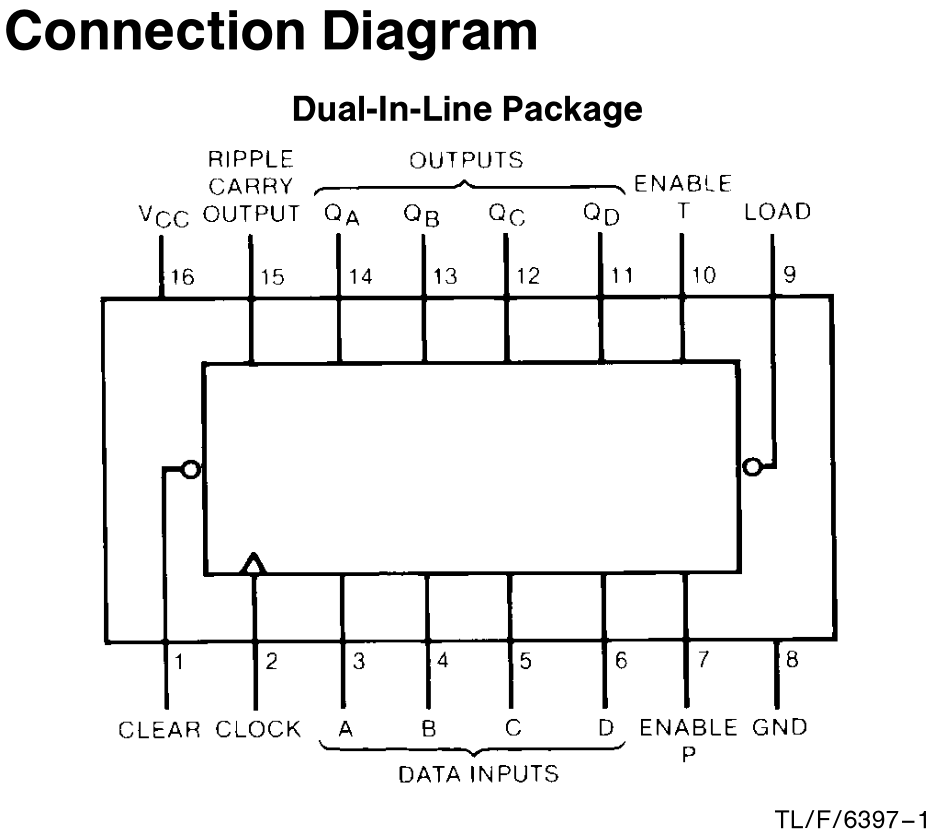
\includegraphics[width=.5\linewidth]{74LS161002.png}
	\caption{74LS161引脚图}
	\label{fig:74LS161引脚图}
\end{figure}

74LS161逻辑功能如表\ref{tab:74LS161逻辑表}所示。

\begin{table}[htbp]
	\centering
	\caption{74LS161逻辑表}
	\label{tab:74LS161逻辑表}
	\begin{longtabu}to\linewidth{@{}X[c,1.5]|X[c]X[c]X[c]X[c]X[c]X[c]X[c]X[c]X[c]|X[c]X[c]X[c]X[c]X[c]@{}}
		\toprule
			 & \multicolumn{9}{c}{输入}  & \multicolumn{5}{c}{输出} \\
			 \midrule
			 & CP & $ \overline{Cr}  $  & $ \overline{LD}  $  & $ S_1 $  & $ S_0 $  & $ D $  & $ C $  & $ B $  & $ A $  & $ Q_D $  & $ Q_C $  & $ Q_B $  & $ Q_A $  & $ Q_{CC} $ \\
			 \midrule
		清零 & $ x $ & $ 0 $ & $ x $ & $ x $ & $ x $ & $ x $ & $ x $ & $ x $ & $ x $ & $ 0 $ & $ 0 $ & $ 0 $ & $ 0 $ & $ 0 $\\
		送数 & $ \uparrow $  & $ 1 $ & $ 0 $ & $ 1 $ & $ 1 $ & D & c & b & a & d & c & b & a & \mbox{$ 0-1 $}\\
		计数 & $ \uparrow $ & $ 1 $ & $ 1 $ & $ 1 $ & $ 1 $ & $ x $ & $ x $ & $ x $ & $ x $ & \multicolumn{5}{c}{二进制加法计数}\\
		保持 & $ x $ & $ 1 $ & $ 1 $ & $ 0 $ & $ 1 $ & $ x $ & $ x $ & $ x $ & $ x $ & \multicolumn{5}{c}{不变}\\
		保持 & $ x $ & $ 1 $ & $ 1 $ & $ 1 $ & $ 0 $ & $ x $ & $ x $ & $ x $ & $ x $ & \multicolumn{5}{c}{不变}\\
		\bottomrule
	\end{longtabu}
\end{table}

\begin{description}
	\item[CP:] 计数器脉冲输入端,上升沿触发;
	\item[$ \overline{Cr}  $:] 异步淸零端(复位端),低电平有效;
	\item[$ A,B,C,D $:] 预置数并入数搞输入端;
	\item[$ \overline{LD} $:] 同步预置数据控制端,低电平有效。当控制端有效时。在时钟脉冲作用下,一次件将并入口数据送到输出口;
	\item[$ S_1,S_0 $ :] 工作状态使能端,当时,$ S_1S_0=0 $,则计数器处于保持状态。$ S_1S_0=1 $,则计数器处于加法计数状态;
	\item[$ Q_d,Q_c,Q_e,Q_a $:] 计数器四位输出端;
	\item[$ Q_cc $:] 进位输出端,当$ Q_DQ_CQ_BQ_A=1 $ 时,$ Q_cc $端输出髙电平。
\end{description}

\subsection{双四位同步BCD码加法计数器}%
\label{sub:}

双四位同步BCD码加法计数器CD4518逻辑图如图\ref{fig:CD4518逻辑图}与局部引脚图如图\ref{fig:CD4518引脚图}。

\begin{figure}[htpb]
	\centering
	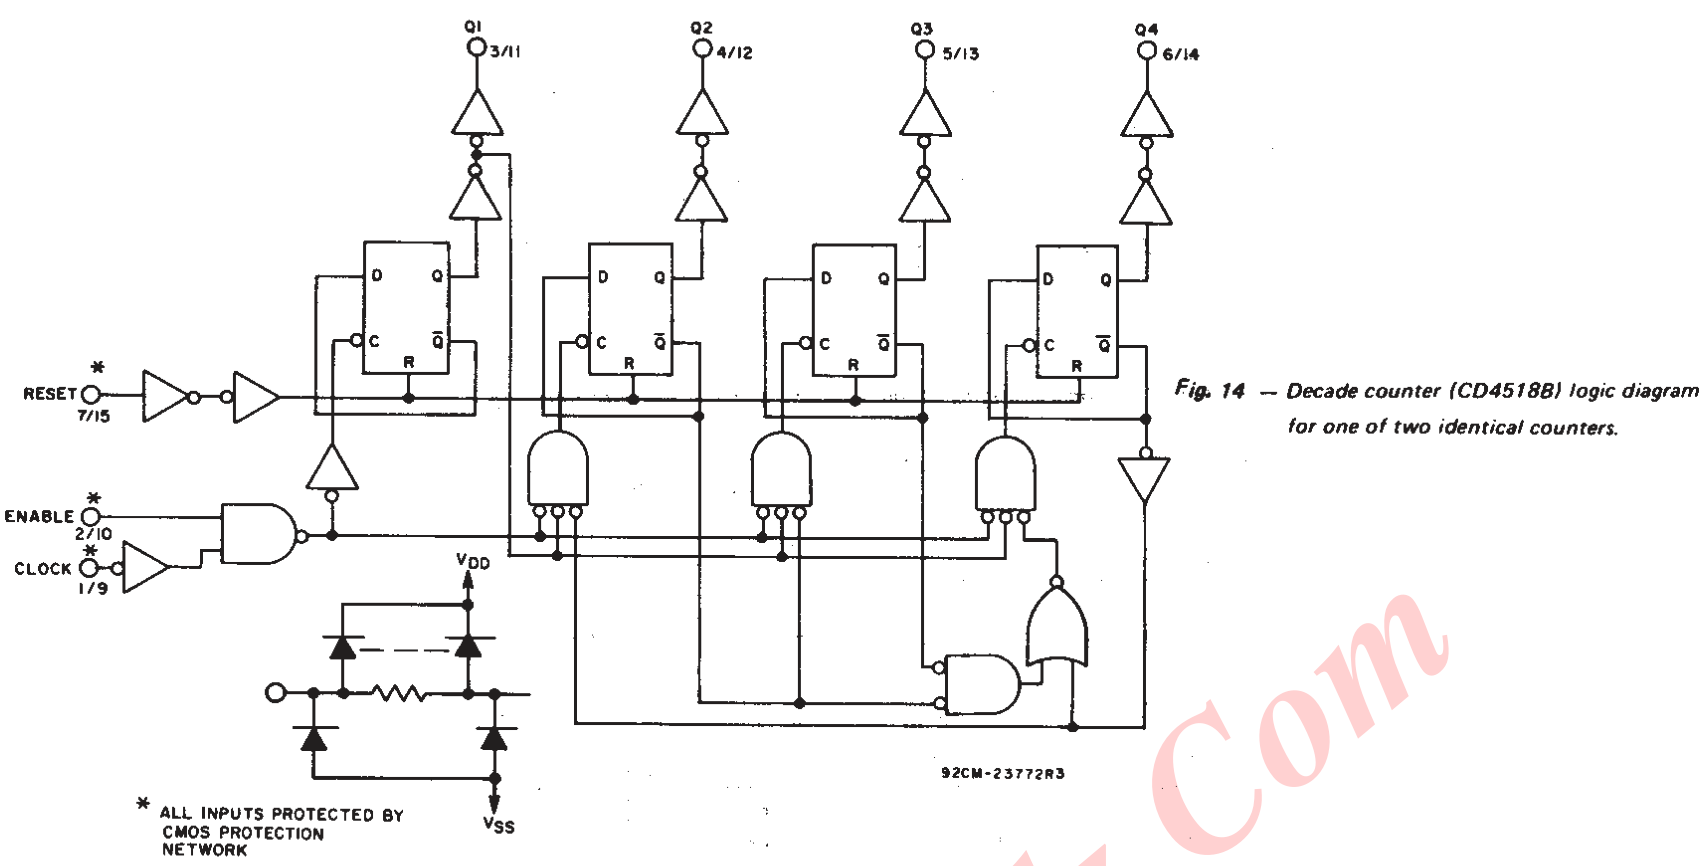
\includegraphics[width=0.8\linewidth]{CD4518001.png}
	\caption{CD4518逻辑图}
	\label{fig:CD4518逻辑图}
\end{figure}

\begin{figure}[htpb]
	\centering
	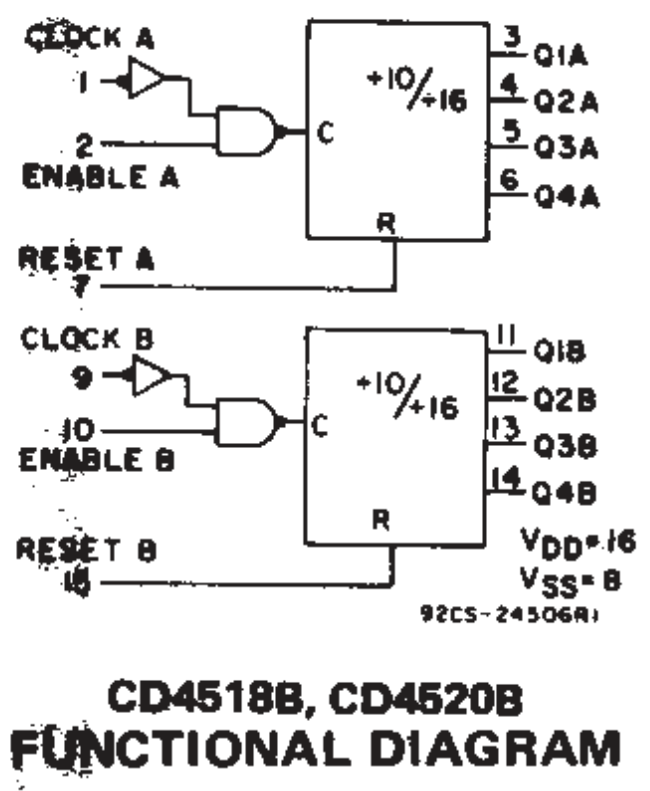
\includegraphics[width=0.5\linewidth]{CD4518002.png}
	\caption{CD4518引脚图}
	\label{fig:CD4518引脚图}
\end{figure}

\newpage
CD4518逻辑功能如表\ref{tab:CD4518逻辑表}所示。

\begin{table}[htbp]
	\centering
	\caption{CD4518逻辑表}
	\label{tab:CD4518逻辑表}
	\begin{longtabu}to\linewidth{@{}X[c]|X[c]X[c]X[c]|X[c]X[c]X[c]X[c]@{}}
		\toprule
		&$ \overline{Cr}  $ &CP&EN &$ Q_d $& $ Q_c $& $ Q_b $& $ Q_a $
		\\
		\midrule
		清零 & $1$ & $x$ & $x$ & $0$ & $0$ & $0$ & $0$
		\\
		计数 & $0$ & $\uparrow$ & $1$ & \multicolumn{4}{c}{BCD码加法计数}
		\\
		保持 & $0$ & $x$ & $0$ & \multicolumn{4}{c}{保持}
		\\
		计数 & $0$ & $0$ & $\downarrow$ & \multicolumn{4}{c}{BCD码减法计数}
		\\
		保持 & $0$ & $1$ & $x$ & \multicolumn{4}{c}{保持}
		\\
		\bottomrule
	\end{longtabu}
\end{table}

\begin{description}
	\item[Cr:] 异步清零端(复位端),高电平有效;
	\item[CP,EN:] 计数器工作状态控制与时钟脉冲输入端;
	\item[$ Q_a,Q_c,Q_e,Q_a $:] 计数器四位数据输出端。
\end{description}

\subsection{计数器工作状态区间控制方法}%
\label{sub:计数器工作状态区间控制方法}

计数器模式控制工作状态区间有两种控制方法:一种是置位(预置数)法,一种是复位(清零)法。如试设计一模式为m的计数器,用置数法时在计数器为m-1时,将输出端高有效为“1”的端口数据取出经(门电路)控制器接至计数器的同步置数端,并准备好并入数据.等吋钟来到使计数器回到起始状态(如遇y异步预置数据控制时,计数器定位在m时的状态,不需等时钟来到使计数器回到起始状态)。用复位法时在计数器为m时,将输出端高有效为“1”的端口数据取出经(门电路)控制器接至计数器的异步复位端(如同步复位控制时,计数器定位在m-1时的状态,等时钟来到)。使计数器回到起始0状态。在多个计数器组合工作时,先将计数器工作设计控制在最大工作循环下,在按计数器模式控制的控制方法,把计数器控制在所需的工作状态下。二进制代码——十六进制代码转换表如表\ref{tab:二进制代码——十六进制码转换表}所示。

\begin{table}[htbp]
	\centering
	\caption{二进制代码——十六进制码转换表}
	\label{tab:二进制代码——十六进制码转换表}
	\csvreader[
	head to column names,
	tabular=c|cccc|c|cccc,
	table head=
	\toprule
	十六进制码 & \multicolumn{4}{c|}{二进制代码} & 十六进制码 & \multicolumn{4}{c}{二进制代码}
	\\
	\midrule
			   &$Q_D$&$Q_C$&$Q_B$&$Q_A$&&$Q_D$&$Q_C$&$Q_B$&$Q_A$
			   \\
			   \midrule,
			   table foot=\bottomrule
			   ]{src/2to16.csv}{}{
	\1&\2&\3&\4&\5&\6&\7&\8&\9&\0
}
\end{table}

\newpage
\section{实验步骤及结果}%
\label{sec:实验步骤及结果\arabic{chapter}}

\subsection{用74LS161四位二进制计数器设计完成$ 0..5\rightarrow A..D\rightarrow 0 $区间计数器}%
\label{sub:用74LS161四位二进制计数器设计完成区间计数器}

\begin{align}
	\overline{\mathrm{LD}} &= \overline{Q_2Q_0}\\
	(D_3D_2D_1D_0)_{(2)} &= (0 \overline{Q_3}0 \overline{Q_3} )_{(2)}
\end{align}

\begin{figure}[htpb]
	\centering
	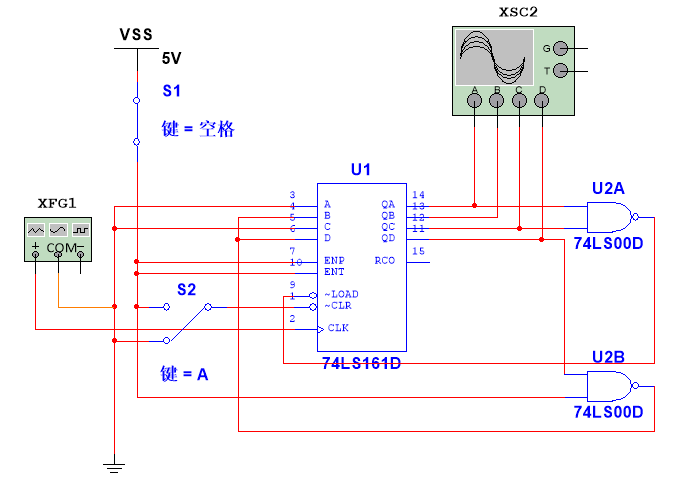
\includegraphics[width=0.8\linewidth]{321.png}
	\caption{计数器设计连线图}
	\label{fig:计数器设计连线图}
\end{figure}

\begin{figure}[htpb]
	\centering
	\begin{subfigure}[htpb]{.45\linewidth}
		\centering
		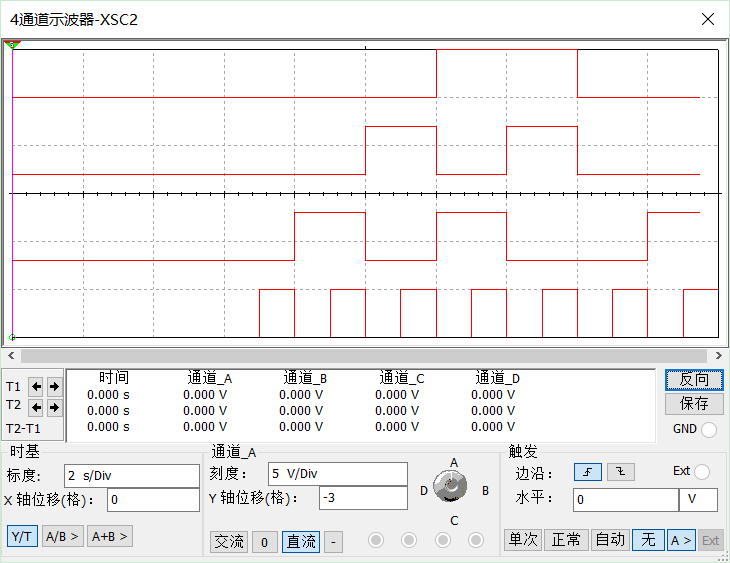
\includegraphics[width=\linewidth]{322.png}
		\caption{计数器仿真结果}
		\label{fig:计数器仿真结果}
	\end{subfigure}
	\quad
	\begin{subfigure}[htpb]{.45\linewidth}
		\centering
		\includegraphics[width=\linewidth]{323.jpg}
		\caption{计数器实验结果}
		\label{fig:计数器实验结果}
	\end{subfigure}
	\caption{计数器结果}
	\label{fig:计数器结果}
\end{figure}

\newpage

\subsection{绘制CD4518BCD码计数器工作波形}%
\label{sub:绘制CD4518BCD码计数器工作波形}

\begin{figure}[htpb]
	\centering
	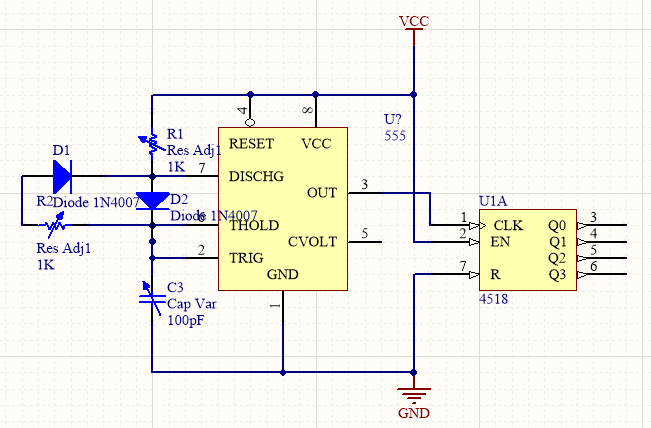
\includegraphics[width=\linewidth]{341.png}
	\caption{CD4518BCD码计数器设计连线图}
	\label{fig:CD4518BCD码计数器设计连线图}
\end{figure}

\section{实验思考}%
\label{sec:实验思考\arabic{chapter}}

\begin{enumerate}
	\item 用CD4518BCD码计数器实现模24计数器能用几种方法,试拿出实现计数器的逻辑图。
\end{enumerate}

CD4518内含2个BCD码加法计数器,可以将2个计数器级联成$ 6\times 4 $、$ 4\times 6 $、$ 3\times 8 $、$ 8\times 3 $的模24计数器,也可以级联成$ 10\times 10 $的模100计数器,计数到24时异步清零;实质上可以级联成任何模大于24的计数器计数到24时异步清零。

\begin{figure}[htpb]
	\centering
	\begin{subfigure}[htpb]{.45\linewidth}
		\centering
		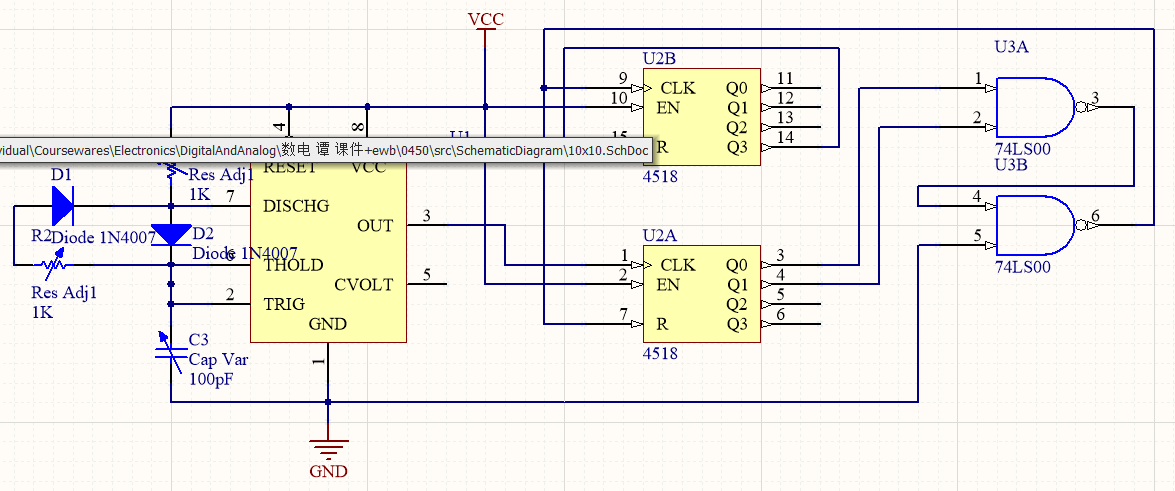
\includegraphics[width=\linewidth]{3x8.png}
		\caption{模24计数器设计连线图3x8}
		\label{fig:模24计数器设计连线图3x8}
	\end{subfigure}
	\quad
	\begin{subfigure}[htpb]{.45\linewidth}
		\centering
		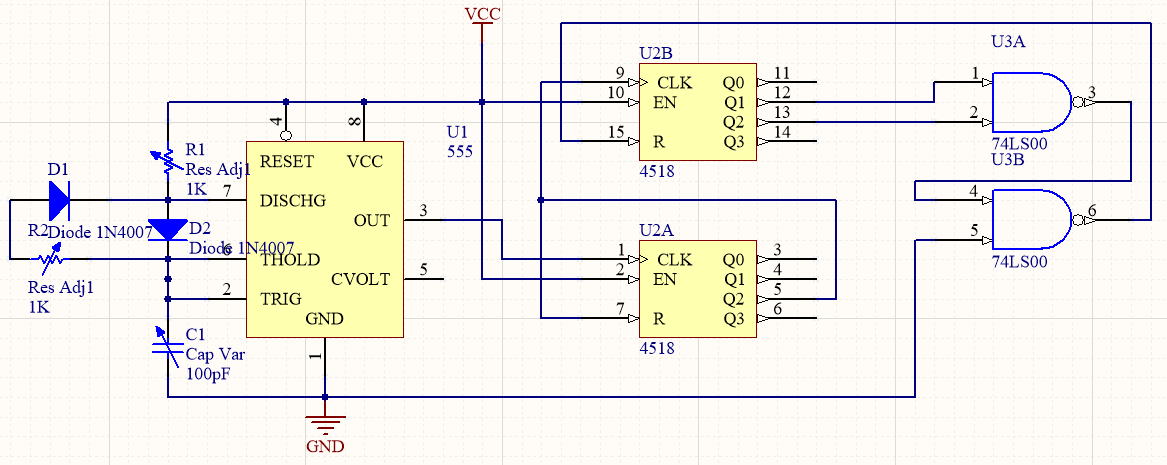
\includegraphics[width=\linewidth]{4x6.png}
		\caption{模24计数器设计连线图4x6}
		\label{fig:模24计数器设计连线图4x6}
	\end{subfigure}

	\begin{subfigure}[htpb]{.45\linewidth}
		\centering
		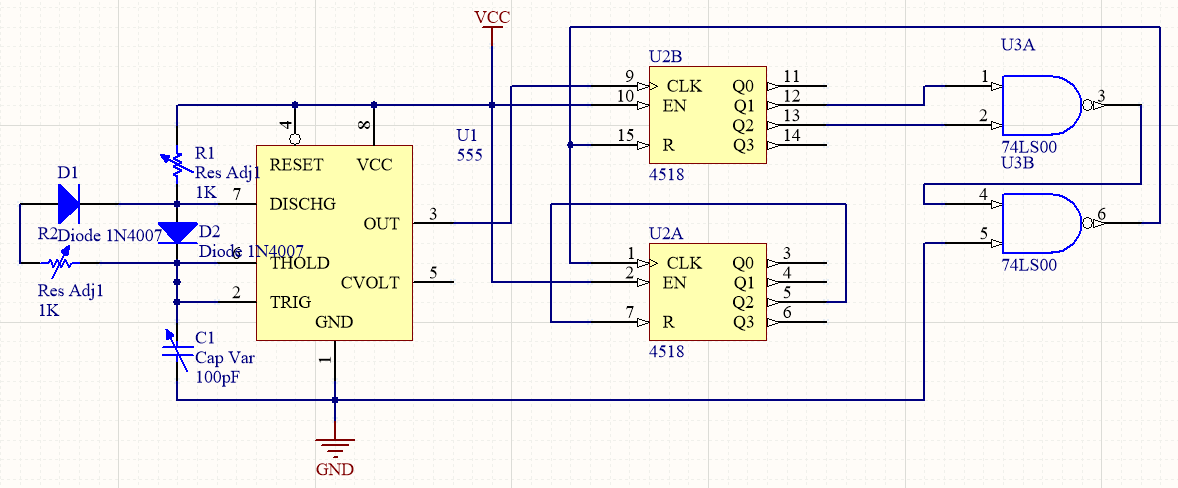
\includegraphics[width=\linewidth]{6x4.png}
		\caption{模24计数器设计连线图6x4}
		\label{fig:模24计数器设计连线图6x4}
	\end{subfigure}
	\quad
	\begin{subfigure}[htpb]{.45\linewidth}
		\centering
		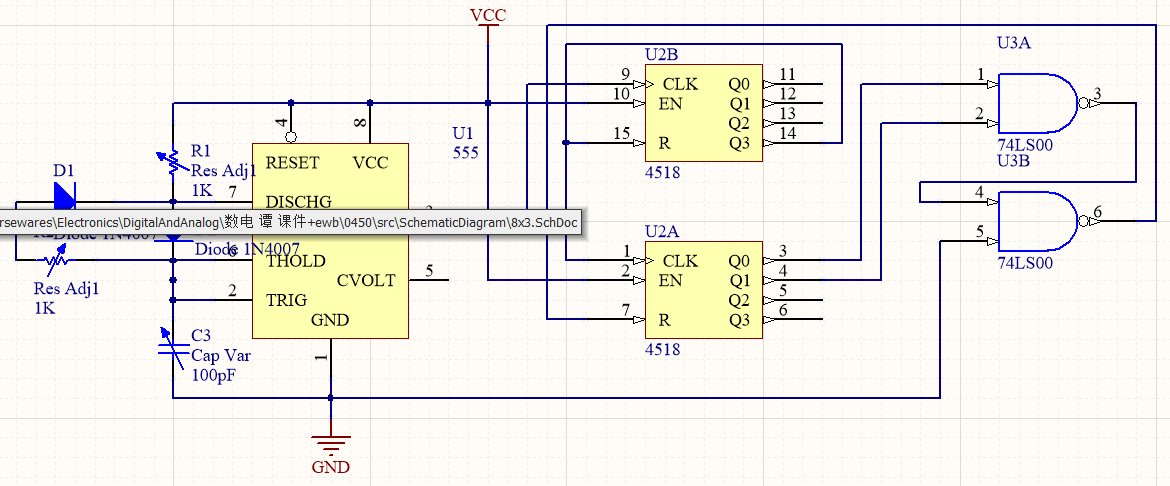
\includegraphics[width=\linewidth]{8x3.png}
		\caption{模24计数器设计连线图8x3}
		\label{fig:模24计数器设计连线图8x3}
	\end{subfigure}

	\begin{subfigure}[htpb]{\linewidth}
		\centering
		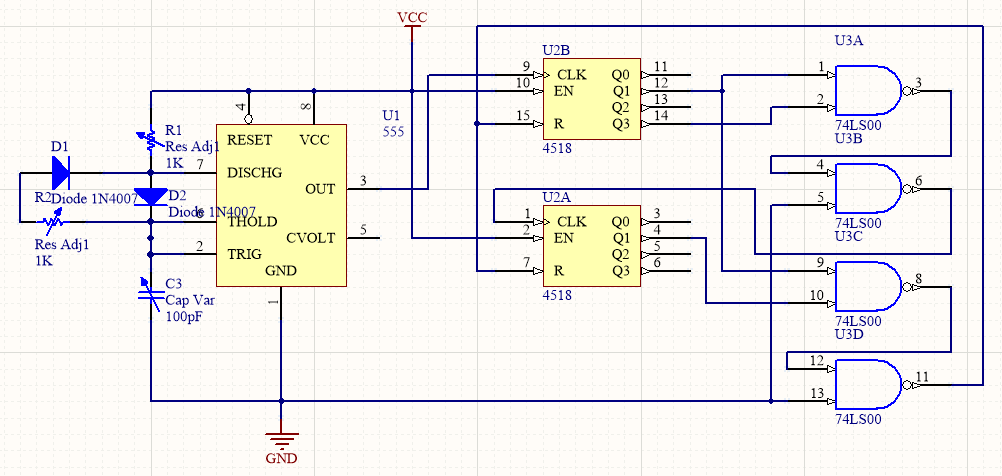
\includegraphics[width=\linewidth]{10x10.png}
		\caption{模24计数器设计连线图10x10}
		\label{fig:模24计数器设计连线图10x10}
	\end{subfigure}
	\caption{模24计数器设计连线图}
	\label{fig:模24计数器设计连线图}
\end{figure}

\chapter{移位寄存器及应用}%
\label{cha:移位寄存器及应用}

\section{实验目的}%
\label{sec:实验目的}

掌握移位寄存器的逻辑功能及应用。

\section{实验要求}%
\label{sec:实验要求}

用移位寄存器实现循环工作和分频器工作。并绘制分频器工作波形。

\begin{enumerate}
	\item 绘制74LS194芯片的逻辑功能;
	\item 绘制实验内容2的实验电路并阐述设计方法及测试流程;
	\item 绘制实验内容5的实验电路及波形图并阐述设计方法;
	\item 格式及其他内容参考实验报告模版。
\end{enumerate}

\section{实验内容}%
\label{sec:实验内容}

\begin{enumerate}
	\item 按表\ref{tab:74LS194四位双向移位寄存器逻辑功能表}测试74LS194四位双向移位寄存器逻辑功能;
	\item 用74LS194设计实现(自启动)左、右循环计数,状态如图\ref{fig:左、右循环计数状态转换图};

		\begin{figure}[htpb]
			\centering
			% 流程图定义基本形状
			\tikzstyle{startstop} = [rectangle, rounded corners, minimum width = 2cm, minimum height=1cm,text centered, draw = black, fill = red!40]
			\tikzstyle{io} = [trapezium, trapezium left angle=70, trapezium right angle=110, minimum width=2cm, minimum height=1cm, text centered, draw=black, fill = blue!40]
			\tikzstyle{process} = [rectangle, minimum width=3cm, minimum height=1cm, text centered, draw=black, fill = yellow!50]
			\tikzstyle{decision} = [diamond, aspect = 3, text centered, draw=black, fill = green!30]
			% 箭头形式
			\tikzstyle{arrow} = [->,>=stealth]
			\begin{tikzpicture}[node distance=2cm]
				%定义流程图具体形状
				\node (0001) {0001};
				\node (0010) [right of=0001] {0010};
				\node (0100) [right of=0010] {0100};
				\node (1000) [right of=0100] {1000};
				%连接具体形状
				\draw [arrow](0001) --  (0010);
				\draw [arrow](0010) --  (0100);
				\draw [arrow](0100) --  (1000);
				\draw [arrow](1000) |- ($(0001) + (0,-1)$ )node[anchor=west] {}-- (0001);
			\end{tikzpicture}
			\caption{左、右循环计数状态转换图}
			\label{fig:左、右循环计数状态转换图}
		\end{figure}

	\item 用74LS194设计实现(无自启动)扭环计数,状态如图\ref{fig:扭环计数状态转换图};

		\begin{figure}[htpb]
			\centering
			% 流程图定义基本形状
			\tikzstyle{startstop} = [rectangle, rounded corners, minimum width = 2cm, minimum height=1cm,text centered, draw = black, fill = red!40]
			\tikzstyle{io} = [trapezium, trapezium left angle=70, trapezium right angle=110, minimum width=2cm, minimum height=1cm, text centered, draw=black, fill = blue!40]
			\tikzstyle{process} = [rectangle, minimum width=3cm, minimum height=1cm, text centered, draw=black, fill = yellow!50]
			\tikzstyle{decision} = [diamond, aspect = 3, text centered, draw=black, fill = green!30]
			% 箭头形式
			\tikzstyle{arrow} = [->,>=stealth]
			\begin{tikzpicture}[node distance=2cm]
				%定义流程图具体形状
				\node (0000)  {0000};
				\node (0001) [right of=0000] {0001};
				\node (0011) [right of=0001] {0011};
				\node (0111) [right of=0011] {0111};
				\node (1111) [right of=0111] {1111};
				\node (1110) [right of=1111] {1110};
				\node (1100) [right of=1110] {1100};
				\node (1000) [right of=1100] {1000};
				%连接具体形状
				\draw [arrow](0000) -- (0001);
				\draw [arrow](0001) -- (0011);
				\draw [arrow](0011) -- (0111);
				\draw [arrow](0111) -- (1111);
				\draw [arrow](1111) -- (1110);
				\draw [arrow](1110) -- (1100);
				\draw [arrow](1100) -- (1000);
				\draw [arrow](1000) |- ($(0000) + (0,-1)$ )node[anchor=west] {} -- (0000);
			\end{tikzpicture}
			\caption{扭环计数状态转换图}
			\label{fig:扭环计数状态转换图}
		\end{figure}
	\item 用74LS194实现$ M=2^n-1 $ 最大长度计数,反馈表达式为$ D_{SR}=Q_3\oplus Q_2 $,观察并记录计数器循环状态(无自启动);
	\item 用74LS194设计实现五分频电路,状态如图\ref{fig:五分频电路状态图}。通过示波器绘制工作波形。

		\begin{figure}[htpb]
			\centering
			% 流程图定义基本形状
			\tikzstyle{startstop} = [rectangle, rounded corners, minimum width = 2cm, minimum height=1cm,text centered, draw = black, fill = red!40]
			\tikzstyle{io} = [trapezium, trapezium left angle=70, trapezium right angle=110, minimum width=2cm, minimum height=1cm, text centered, draw=black, fill = blue!40]
			\tikzstyle{process} = [rectangle, minimum width=3cm, minimum height=1cm, text centered, draw=black, fill = yellow!50]
			\tikzstyle{decision} = [diamond, aspect = 3, text centered, draw=black, fill = green!30]
			% 箭头形式
			\tikzstyle{arrow} = [->,>=stealth]
			\begin{tikzpicture}[node distance=2cm]
				%定义流程图具体形状
				\node (1100)  {1100};
				\node (1001) [right of=1100] {1001};
				\node (0011) [right of=1001] {0011};
				\node (0111) [right of=0011] {0111};
				\node (1110) [right of=0111] {1110};
				%连接具体形状
				\draw [arrow](1100) -- (1001);
				\draw [arrow](1001) -- (0011);
				\draw [arrow](0011) -- (0111);
				\draw [arrow](0111) -- (1110);
				\draw [arrow](1110) |- ($(1100) + (0,-1)$ )node[anchor=west] {}-- (1100);
			\end{tikzpicture}
			\caption{五分频电路状态图}
			\label{fig:五分频电路状态图}
		\end{figure}

	\item 设计实现50\%占空比的五分频电路,通过示波器绘制工作波形。
\end{enumerate}

\section{实验原理}%
\label{sec:实验原理}

74LS194四位双向移位寄存器逻辑图与引脚部局图如图\ref{fig:74LS194逻辑图}和\ref{fig:74LS194引脚图}。

\begin{figure}[htpb]
	\centering
	\begin{subfigure}[htpb]{.45\linewidth}
		\centering
		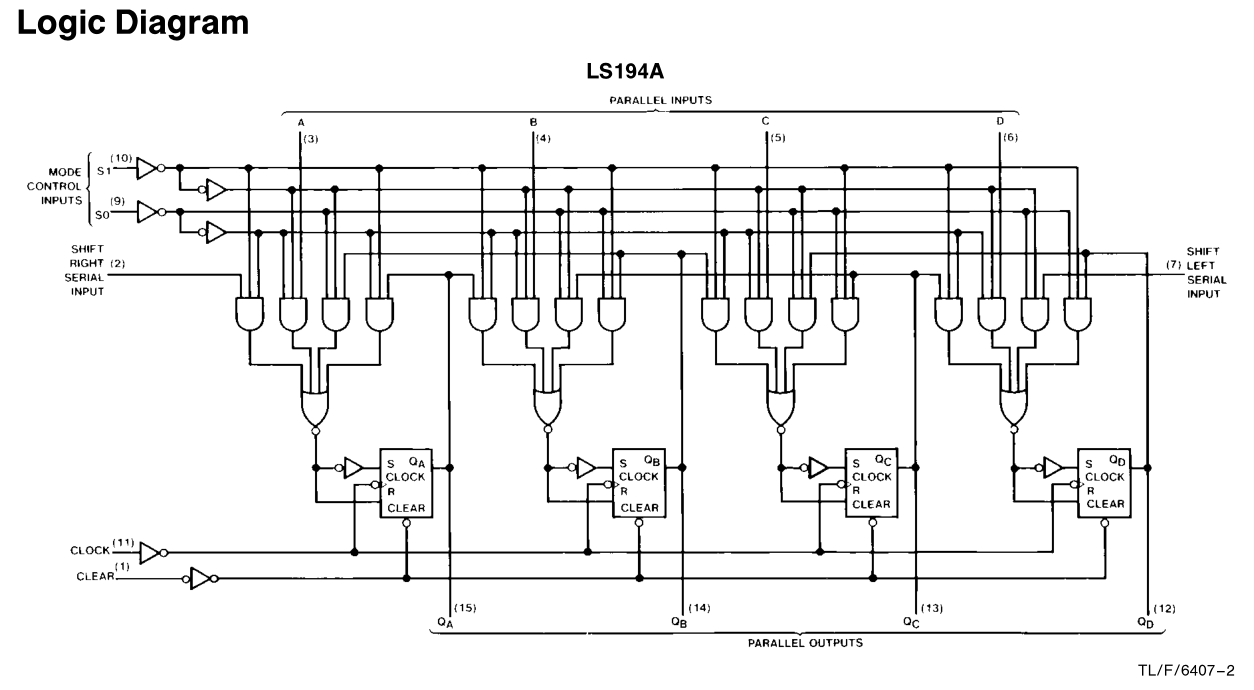
\includegraphics[width=\linewidth]{74LS194002.png}
		\caption{74LS194逻辑图}
		\label{fig:74LS194逻辑图}
	\end{subfigure}
	\quad
	\begin{subfigure}[htpb]{.45\linewidth}
		\centering
		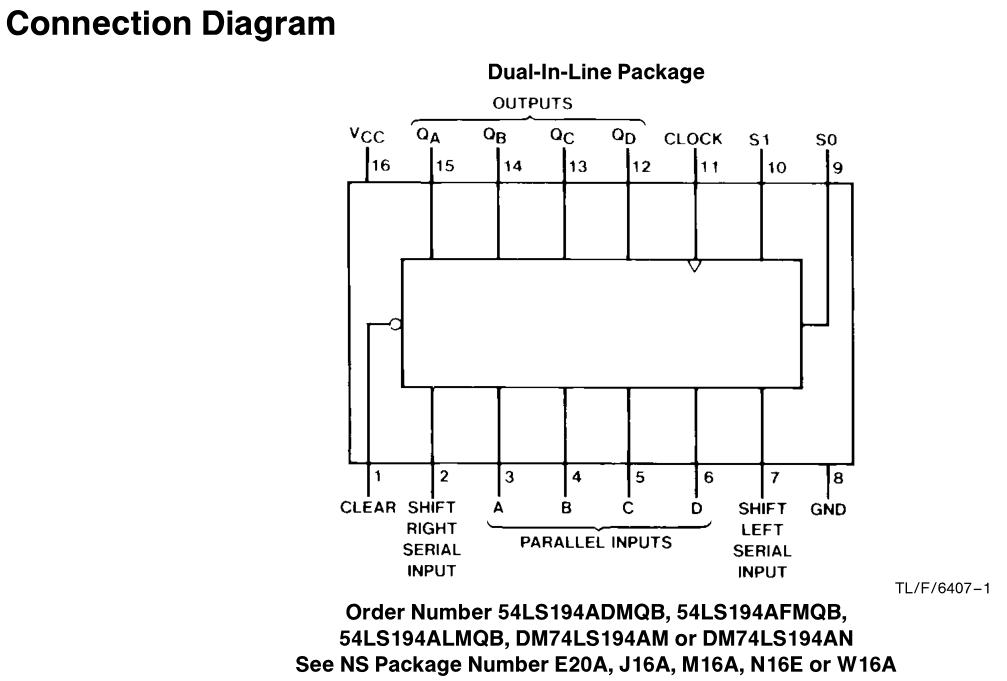
\includegraphics[width=\linewidth]{74LS194001.png}
		\caption{74LS194引脚图}
		\label{fig:74LS194引脚图}
	\end{subfigure}
	\caption{74LS194逻辑图和引脚图}
	\label{fig:74LS194逻辑图和引脚图}
\end{figure}

74LS194四位双向移位寄存器结构为四个主从RS触发器(已经转换成D触发器)与一些门电路组成。

\begin{description}
	\item[Cr:]为异步清零端,低电平有效;
	\item[CP:]为时钟脉冲输入端,上升沿有效;
	\item[DSR:]为右移串行数据输入端;
	\item[DSL:]为左移串行数据输入端;
	\item[MB,MA:]为移位寄存器工作状态控制端,有四种状态可使用;
	\item[$ Q_1,Q_2,Q_3,Q_4 $:]寄存器四位输出端。
\end{description}

74LS194四位双向移位寄存器逻辑功能如表\ref{tab:74LS194四位双向移位寄存器逻辑功能表}所示。

\begin{table}[htpb]
	\centering
	\caption{74LS194四位双向移位寄存器逻辑功能表}
	\label{tab:74LS194四位双向移位寄存器逻辑功能表}
	\begin{tabu}to\linewidth{|X[c,1.5]|X[c]X[c]X[c]X[c]X[c]X[c]X[c]X[c]X[c]X[c]|X[c]X[c]X[c]X[c]|}
		\hline
							   & Cr & CP & MB & MA & DSL & DSR & D3 & D2 & D1 & D0 & Q3 & Q2 & Q1 & Q0
							   \\
							   \hline
		清零                   & 0  & X  & X  & X  & X   & X   & X  & X  & X  & X  & 0  & 0  & 0  & 0
		\\
		保持                   & 1  & X  & 0  & 0  & X   & X   & X  & X  & X  & X  & \multicolumn{4}{c|}{不变}
		\\
		\multirow{2}{*}{右移}  & 1  & ↑  & 0  & 1  & X   & 0   & X  & X  & X  & X  & Q2 & Q1 & Q0 & 0
		\\
							   & 1  & ↑  & 0  & 1  & X   & 1   & X  & X  & X  & X  & Q2 & Q1 & Q0 & 1
							   \\
		\multirow{2}{*}{左移}  & 1  & ↑  & 1  & 0  & 0   & X   & X  & X  & X  & X  & 0  & Q3 & Q2 & Q1
		\\
							   & 1  & ↑  & 1  & 0  & 1   & X   & X  & X  & X  & X  & 1  & Q3 & Q2 & Q1
							   \\
		送数                   & 1  & ↑  & 1  & 1  & X   & X   & d3 & d2 & d1 & d0 & d3 & d2 & d1 & d0
		\\
		\hline
	\end{tabu}
\end{table}

由于移位寄存器使用D触发器组成。在移位寄存器工作时,串入口所需的数据即为第一个得到数据的输出端所需的数据。设计中可根据已知的循环状态,找出串入口的数据需求。即可在卡诺图中进行转换,得到设计电路所需参数,达到电路设计目的。需注意到电路的自启动的问题,以保证电路在特殊场合下都能完成任务。

例:设计一个四位彩灯控制器,循环使每个彩灯轮流点亮一次。首先需拿出实现电路的状态转换图,设灯亮为“1”,灭灯为“0”,得到循环状态转换图如图\ref{fig:状态转换图}。补足串入口所需状态,再定输出口高低位方向,放在卡诺图\ref{tab:卡诺图}上进行转换,即可得到电路所需参数。实现电路逻辑图如图\ref{fig:四位彩灯控制器电路逻辑图(无自启动)}(因有其它数据不能自动转入循环状态内为无自启动循环方式,简称无自启动)。

\begin{figure}[htpb]
	\centering
	% 流程图定义基本形状
	\tikzstyle{startstop} = [rectangle, rounded corners, minimum width = 2cm, minimum height=1cm,text centered, draw = black, fill = red!40]
	\tikzstyle{io} = [trapezium, trapezium left angle=70, trapezium right angle=110, minimum width=2cm, minimum height=1cm, text centered, draw=black, fill = blue!40]
	\tikzstyle{process} = [rectangle, minimum width=3cm, minimum height=1cm, text centered, draw=black, fill = yellow!50]
	\tikzstyle{decision} = [diamond, aspect = 3, text centered, draw=black, fill = green!30]
	% 箭头形式
	\tikzstyle{arrow} = [->,>=stealth]
	\begin{tikzpicture}[node distance=2cm]
		%定义流程图具体形状
		\node (0001)  {0001};
		\node (0010) [right of=0001] {0010};
		\node (0100) [right of=0010] {0100};
		\node (1000) [right of=0100] {1000};
		%连接具体形状
		\draw [arrow](0001) -- (0010);
		\draw [arrow](0010) -- (0100);
		\draw [arrow](0100) -- (1000);
		\draw [arrow](1000) |- ($(0001) + (0,-1)$ )node[anchor=west] {}-- (0001);
	\end{tikzpicture}
	\caption{状态转换图}
	\label{fig:状态转换图}
\end{figure}

\begin{table}[htpb]
	\centering
	\caption{卡诺图}
	\label{tab:卡诺图}
	\begin{tabu}to.5\linewidth{|X[c,2]|X[c]|X[c]|X[c]|X[c]|}
		\hline
		$ Q_1Q_0/Q_3Q_2 $ & 00 & 01 & 11 & 10
		\\
		\hline
		00 & X & 0 & X & 1
		\\
		\hline
		01 & 0 & X & X & X
		\\
		\hline
		11 & X & X & X & X
		\\
		\hline
		10 & X & X & X & X
		\\
		\hline
	\end{tabu}
\end{table}

\begin{figure}[htpb]
	\centering
	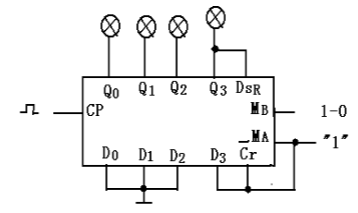
\includegraphics[width=0.5\linewidth]{lamp.png}
	\caption{四位彩灯控制器电路逻辑图(无自启动)}
	\label{fig:四位彩灯控制器电路逻辑图(无自启动)}
\end{figure}

\section{实验步骤及结果}%
\label{sec:实验步骤及结果\arabic{chapter}}

\subsection{用74LS194设计实现(自启动)左、右循环计数}%
\label{sub:用74LS194设计实现(自启动)左、右循环计数}

\begin{align}
	D_\mathrm{SL}=\overline{Q_3}~\overline{Q_2}~\overline{Q_1}= \overline{Q_3 1}~\overline{Q_2 1}~\overline{Q_1 1}
\end{align}

\begin{figure}[htpb]
	\centering
	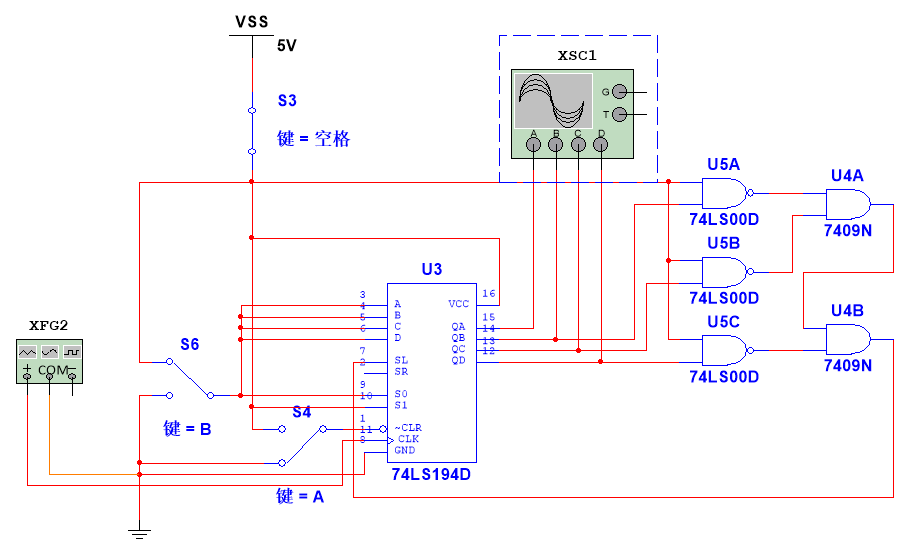
\includegraphics[width=\linewidth]{421.png}
	\caption{循环计数器设计连线图}
	\label{fig:循环计数器设计连线图}
\end{figure}

先把键A按下让清零信号无效,再把键B按下开始左移。

\begin{figure}[htpb]
	\centering
	\begin{subfigure}[htpb]{.45\linewidth}
		\centering
		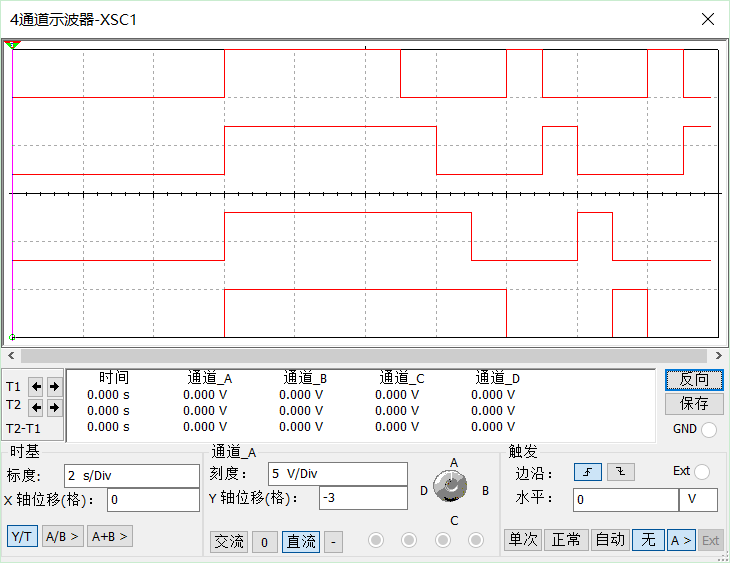
\includegraphics[width=\linewidth]{422.png}
		\caption{循环计数器仿真结果}
		\label{fig:循环计数器仿真结果}
	\end{subfigure}
	\quad
	\begin{subfigure}[htpb]{.45\linewidth}
		\centering
		\includegraphics[width=\linewidth]{423.jpg}
		\caption{循环计数器实验结果}
		\label{fig:循环计数器实验结果}
	\end{subfigure}
	\caption{循环计数器结果}
	\label{fig:循环计数器结果}
\end{figure}

\newpage

\subsection{用74LS194设计实现五分频电路}%
\label{sub:用74LS194设计实现五分频电路}

\begin{align}
	D_\mathrm{SL}= \overline{Q_2}+ \overline{Q_1} \overline{Q_0}= \overline{Q_2 \overline{ \overline{Q_1 1}~\overline{Q_0 1} } }
\end{align}

\begin{figure}[htpb]
	\centering
	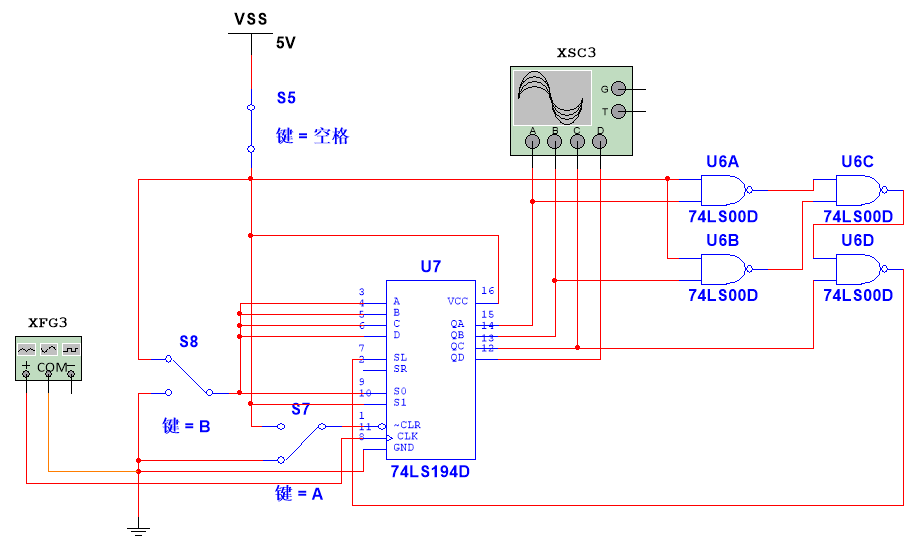
\includegraphics[width=\linewidth]{451.png}
	\caption{五分频电路设计连线图}
	\label{fig:五分频电路设计连线图}
\end{figure}

\begin{figure}[htpb]
	\centering
	\begin{subfigure}[htpb]{.45\linewidth}
		\centering
		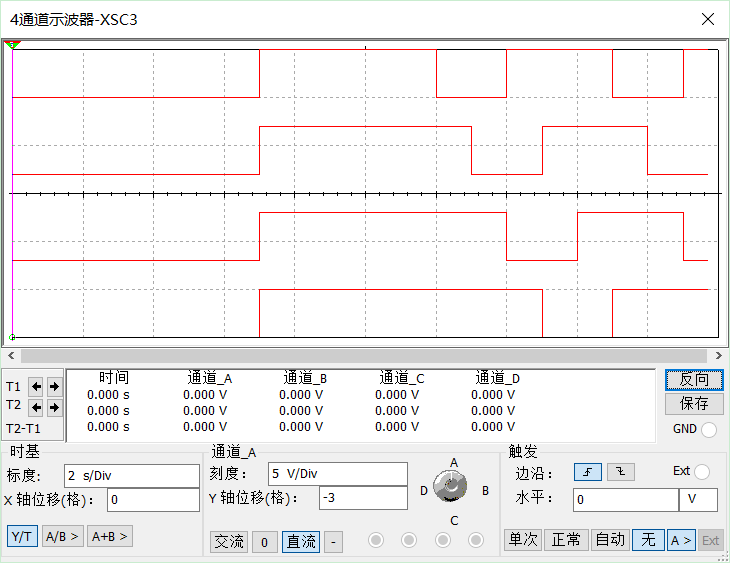
\includegraphics[width=\linewidth]{452.png}
		\caption{五分频电路仿真结果}
		\label{fig:五分频电路仿真结果}
	\end{subfigure}
	\quad
	\begin{subfigure}[htpb]{.45\linewidth}
		\centering
		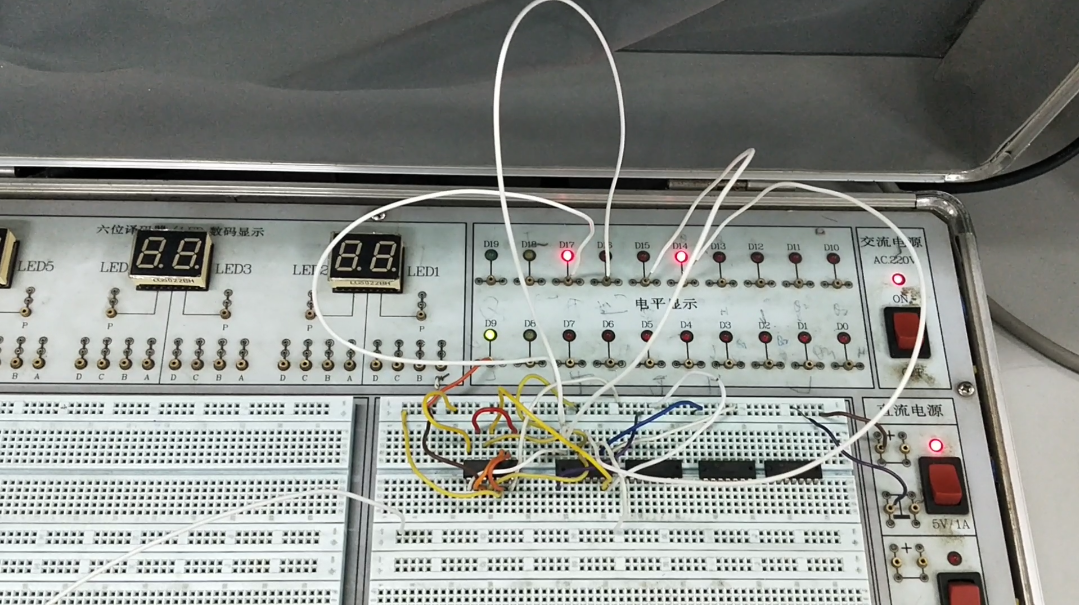
\includegraphics[width=\linewidth]{453.png}
		\caption{五分频电路实验结果}
		\label{fig:五分频电路实验结果}
	\end{subfigure}
	\caption{五分频电路结果}
	\label{fig:五分频电路结果}
\end{figure}

\newpage

\subsection{设计实现50\%占空比的五分频电路}%
\label{sub:设计实现50占空比的五分频电路}

\begin{figure}[htpb]
	\centering
	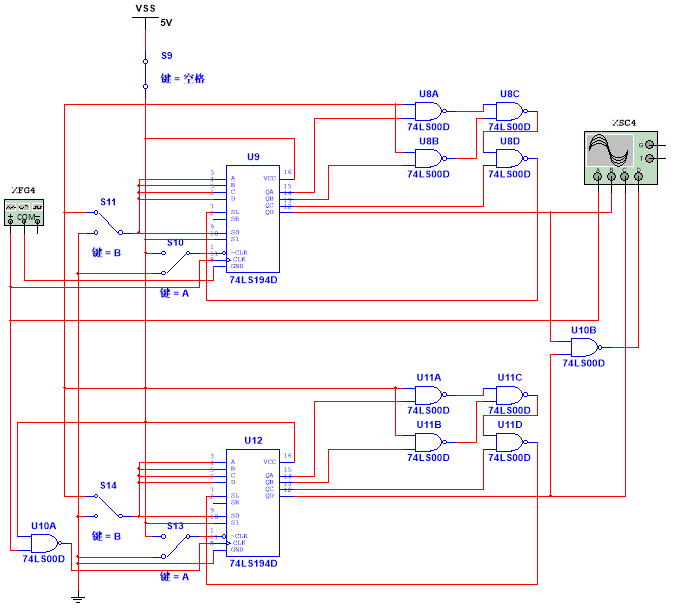
\includegraphics[width=.8\linewidth]{461.png}
	\caption{50\%占空比的五分频电路计数器设计连线图}
	\label{fig:50占空比的五分频电路计数器设计连线图}
\end{figure}

\begin{figure}[htpb]
	\centering
	\begin{subfigure}[htpb]{.45\linewidth}
		\centering
		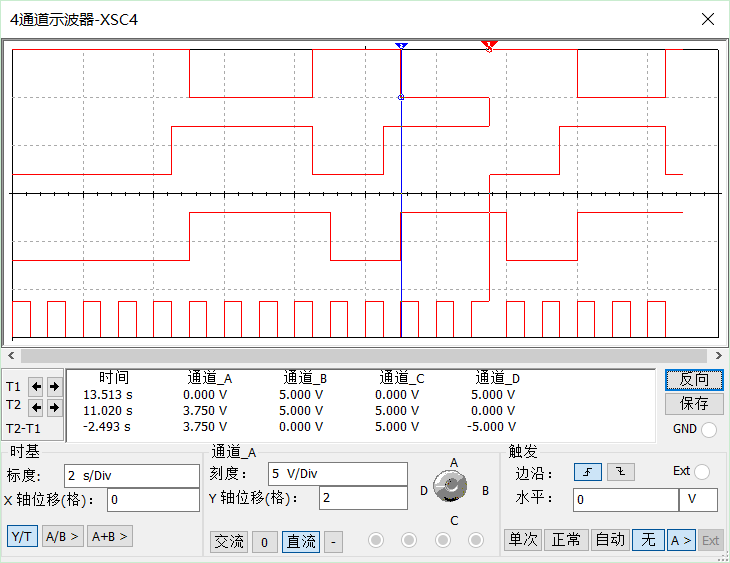
\includegraphics[width=\linewidth]{462.png}
		\caption{50\%占空比的五分频电路仿真结果}
		\label{fig:50占空比的五分频电路仿真结果}
	\end{subfigure}
	\quad
	\begin{subfigure}[htpb]{.45\linewidth}
		\centering
		\includegraphics[width=\linewidth]{463.jpg}
		\caption{50\%占空比的五分频电路实验结果}
		\label{fig:50占空比的五分频电路实验结果}
	\end{subfigure}
	\caption{50\%占空比的五分频电路结果}
	\label{fig:50占空比的五分频电路结果}
\end{figure}

\end{document}

